\documentclass{beamer}

\mode<presentation>
{
 \usetheme{Boadilla}
 \setbeamercovered{transparent}}

\usepackage[english]{babel}
\usepackage{times}

\usepackage{xcolor}
\usepackage{colortbl}
%\usepackage{subfigure}

\usepackage{fontspec} 
\usepackage{xunicode}
\usepackage{xltxtra}
\usepackage{booktabs}
\newenvironment{CJK}{\fontspec[Scale=0.9]{PMingLiU}}{}
\newenvironment{Geeza}{\fontspec[Scale=0.9]{Geeza Pro}}{}

%% for tables
\newcommand{\mc}{\multicolumn}
\newcommand{\lab}[1]{\multicolumn{1}{c}{#1}}
\newcommand{\ind}[1]{{\fboxsep1pt\raisebox{-.5ex}{\fbox{{\tiny #1}}}}}
\newcommand{\IND}[1]{{\fboxsep1pt\raisebox{0ex}{\fbox{{\small #1}}}}}
\newcommand\production[2]{\ensuremath{\langle\mbox{#1}, \mbox{#2}\rangle}}

%% markup
\newcommand{\buffer}[1]{{\color{blue}\textbf{#1}}}
\newcommand{\pred}[1]{\code{#1}}

%% colors
\newcommand{\textred}[1]{\alert{#1}}
\newcommand{\textblue}[1]{\buffer{#1}}
\definecolor{tablecolor}{cmyk}{0,0.3,0.3,0}
\newcommand{\keytab}[1]{\mc{1}{>{\columncolor{tablecolor}}d}{#1}}

% rules
\newcommand{\psr}[2]{#1 $\rightarrow \langle $ #2 $\rangle$}

\newenvironment{unpacked_itemize}{
\begin{itemize}
  \setlength{\itemsep}{10pt}
  \setlength{\parskip}{0pt}
  \setlength{\parsep}{0pt}
}{\end{itemize}}

\newcommand{\condon}{\hspace{0pt} | \hspace{1pt}}
\definecolor{darkblue}{rgb}{0,0,0.6}
\newcommand{\blueexample}[1]{\textcolor{darkblue}{\rm #1}}

%%%%%%%%%%%%%%%%%%%%%%%%%%%%%%%%%%%%%%%%%%%%%%%%%%%%%%%%%%%%%%%%%%%%%%

\newcommand{\ws}{\ensuremath{\vec{w}}}
\newcommand{\pu}{\ensuremath{P_0}}
\newcommand{\bx}{\mathbf{x}}
\newcommand{\bz}{\mathbf{z}}
\newcommand{\bd}{\mathbf{d}}
\newcommand{\by}{\mathbf{y}}
\newcommand\bleu{${B{\scriptstyle LEU}}$}


\title[Models of SCFG Induction]{Models of Synchronous Grammar Induction for SMT}

\author[CLSP Workshop 2010]{
  Workshop 2010
  %Phil Blunsom$^1$ \and Trevor Cohn$^2$ \and Chris Dyer$^3$ \and Adam Lopez$^4$
}

\institute[Baltimore]{
  The Center for Speech and Language Processing \\ Johns Hopkins University
%  $^1$University of Oxford\\ 
%  $^2$University of Sheffield\\ 
%  $^3$Carnegie Mellon University\\ 
%  $^4$University of Edinburgh
}
\date[June 21]{June 21, 2010}

%\subject{Unsupervised models of Synchronous Grammar Induction for SMT}

%\pgfdeclareimage[height=1.0cm]{university-logo}{logo}
%\logo{\pgfuseimage{university-logo}}

%\AtBeginSection[]
%{
%  \begin{frame}<beamer>{Outline}
%    %\tableofcontents[currentsection,currentsubsection]
%    \tableofcontents[currentsection]
%  \end{frame}
%}

%\beamerdefaultoverlayspecification{<+->}

\begin{document}

\begin{frame}
  \titlepage
\end{frame}

%\begin{frame}{Outline}
%  \tableofcontents
% You might wish to add the option [pausesections]
%\end{frame}
 
%\begin{frame}{Outline}
%  \tableofcontents
%  % You might wish to add the option [pausesections]
%\end{frame}


\begin{frame}[t]{Team members}
\begin{center}
{\bf Senior Members} \\
  Phil Blunsom (Oxford)\\
  Trevor Cohn (Sheffield)\\
  Adam Lopez (Edinburgh/COE)\\
  Chris Dyer (CMU)\\
  Jonathan Graehl (ISI)\\
\vspace{0.2in}
{\bf Graduate Students} \\
  Jan Botha (Oxford) \\
  Vladimir Eidelman (Maryland) \\
  Ziyuan Wang (JHU) \\
  ThuyLinh Nguyen (CMU) \\
\vspace{0.2in}
{\bf Undergraduate Students} \\
  Olivia Buzek (Maryland) \\
  Desai Chen (CMU) \\
\end{center}
\end{frame}



\begin{frame}[t]{Statistical machine translation}
%\vspace{1.0cm}
\begin{exampleblock}{Urdu $\rightarrow$ English}
  \begin{figure}
    {\centering 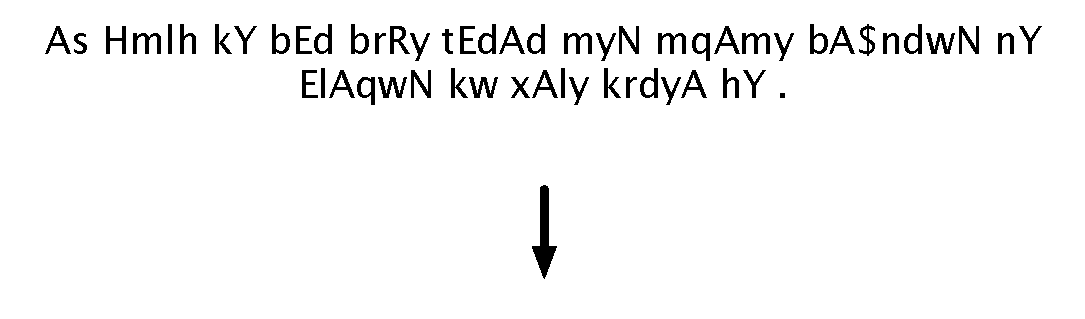
\includegraphics[scale=0.55]{urdu-bw.pdf}}
  \end{figure}
\vspace{0.10cm}
\end{exampleblock}
\begin{itemize}
  \item Statistical machine translation: Learn how to translate from parallel corpora.
\end{itemize}
\end{frame}


\begin{frame}[t]{Statistical machine translation: }
%\vspace{1.0cm}
\begin{exampleblock}{Urdu $\rightarrow$ English}
  \begin{figure}
    {\centering 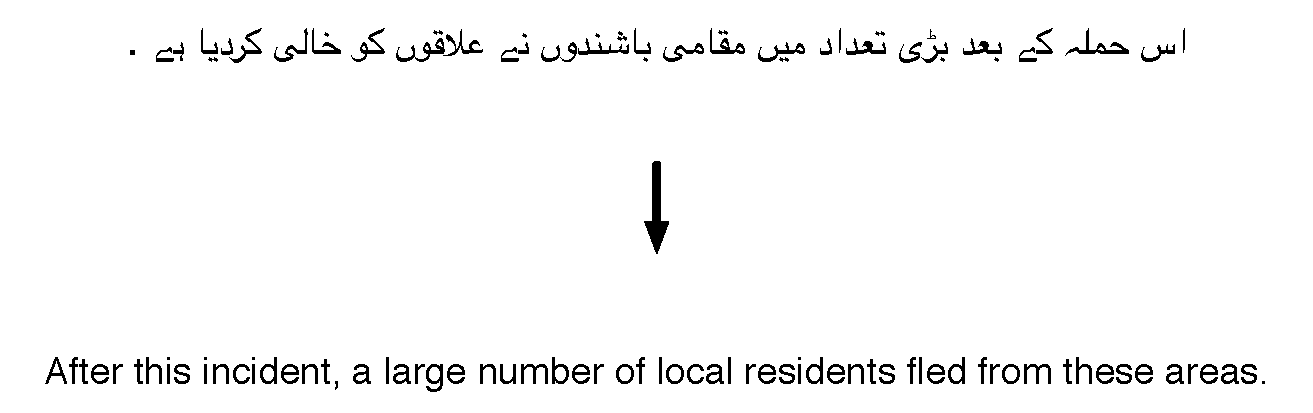
\includegraphics[scale=0.55]{urdu-ref.pdf}}
  \end{figure}
\end{exampleblock}
\begin{itemize}
  \item Statistical machine translation: Learn how to translate from parallel corpora 
\end{itemize}
\end{frame}

\begin{frame}[t]{Statistical machine translation: Before}
%\vspace{1.0cm}
\begin{exampleblock}{Urdu $\rightarrow$ English}
  \begin{figure}
    {\centering 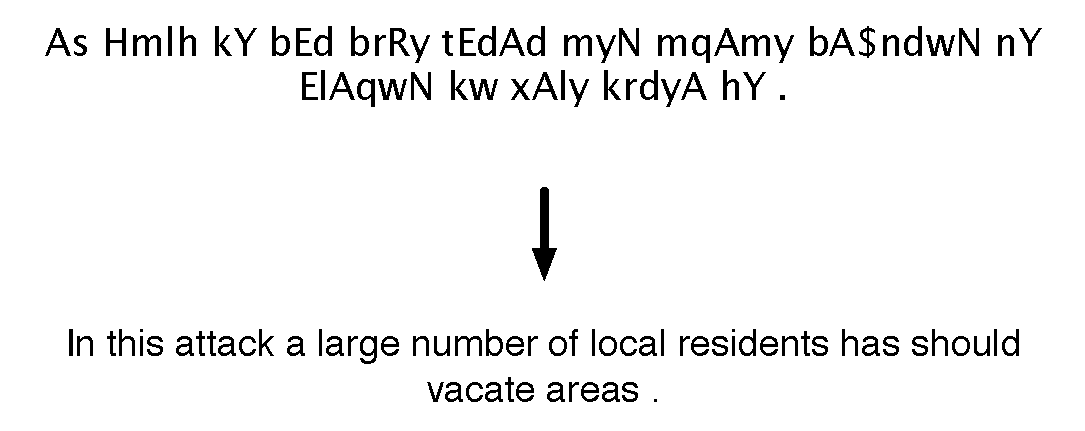
\includegraphics[scale=0.55]{urdu-bl.pdf}}
  \end{figure}
\end{exampleblock}
\begin{itemize}
  \item Current state-of-the-art translation models struggle with language pairs which exhibit large differences in structure.
\end{itemize}
\end{frame}

\begin{frame}[t]{Statistical machine translation: After}
%\vspace{1.0cm}
\begin{exampleblock}{Urdu $\rightarrow$ English}
  \begin{figure}
    {\centering 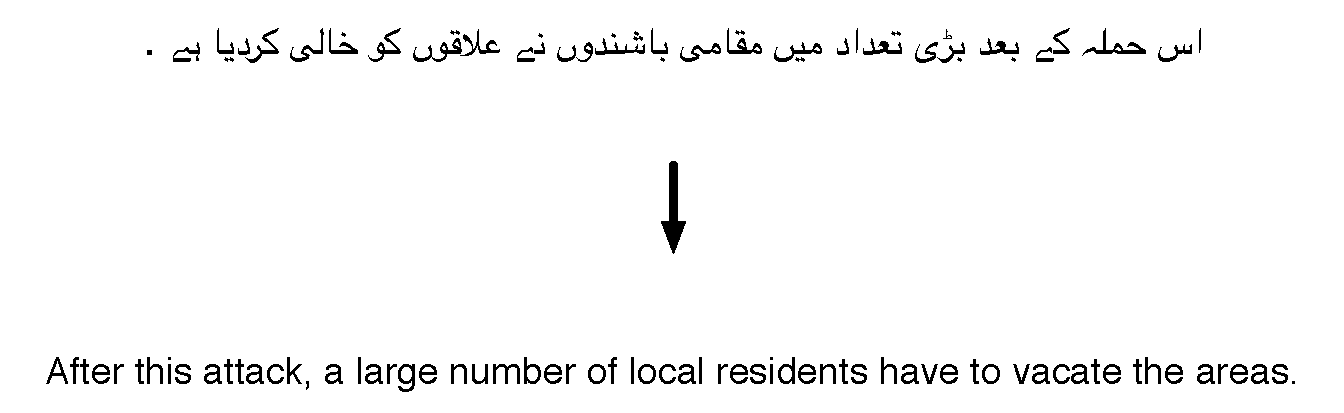
\includegraphics[scale=0.55]{urdu-25hp.pdf}}
  \end{figure}
\end{exampleblock}
\begin{itemize}
  \item In this workshop we've made some small steps towards better translations for difficult language pairs.
\end{itemize}
\end{frame}


\begin{frame}[t]{Statistical machine translation: limitations}
\vspace{1.0cm}
\begin{exampleblock}{Structural divergence between languages:}
  %\vspace{0.3cm}
  \begin{table}
  \centering
    \only<1>{
    \begin{tabular}{|l|l|}
    \hline
      {\bf English}  & {\bf Who wrote this letter?} \\
      \hline
      Arabic   & \begin{Geeza}من الذي كتب هذه الرسالة؟\end{Geeza} \\
               & \textcolor{gray}{(function-word)} (who) (wrote) (this) (the-letter) \\
      \hline
      Chinese  & \begin{CJK}这封  信  是  谁  写  的 ?\end{CJK} \\
               & (this) (letter) (be) (who) (write) (come-from) \textcolor{gray}{(function-word)} \\
      \hline
    \end{tabular}
    }
    \only<2>{
    \begin{tabular}{|l|l|}
    \hline
      {\bf English}  & {\bf \textcolor{blue}{Who} \textcolor{green}{wrote} \textcolor{red}{this} \textcolor{orange}{letter?}} \\
      \hline
      Arabic   & \begin{Geeza}من الذي كتب هذه الرسالة؟\end{Geeza} \\
               & \textcolor{gray}{(function-word)} \textcolor{blue}{(who)} \textcolor{green}{(wrote)} \textcolor{red}{(this)} \textcolor{orange}{(the-letter)} \\
      \hline
      Chinese  & \begin{CJK}这封  信  是  谁  写  的 ?\end{CJK} \\
               & (this) (letter) (be) (who) (write) (come-from) \textcolor{gray}{(function-word)} \\
      \hline
    \end{tabular}
    }
    \only<3->{
    \begin{tabular}{|l|l|}
    \hline
      {\bf English}  & {\bf \textcolor{blue}{Who wrote} \textcolor{red}{this letter}?} \\
      \hline
      Arabic   & \begin{Geeza}من الذي كتب هذه الرسالة؟\end{Geeza} \\
               & \textcolor{gray}{(function-word)} (who) (wrote) (this) (the-letter) \\
      \hline
      Chinese  & \begin{CJK}\textcolor{red}{这封  信}  \textcolor{blue}{是  谁  写}  的 ?\end{CJK} \\
               & \textcolor{red}{(this) (letter)} \textcolor{blue}{(be) (who) (write) (come-from)} \textcolor{gray}{(function-word)} \\
      \hline
    \end{tabular}
  }
  \end{table}
\end{exampleblock}
\only<4>{
  \begin{itemize}
  \item Phrasal translation equivalences \textcolor{green}{(existing models)}
  \item {\bf Constituent reordering \textcolor{blue}{(this workshop!)}}
  \item Morphology \textcolor{red}{(Next year?)}
  \end{itemize}
}
\end{frame}

\begin{frame}[t]{Statistical machine translation: successes}
\begin{center}
  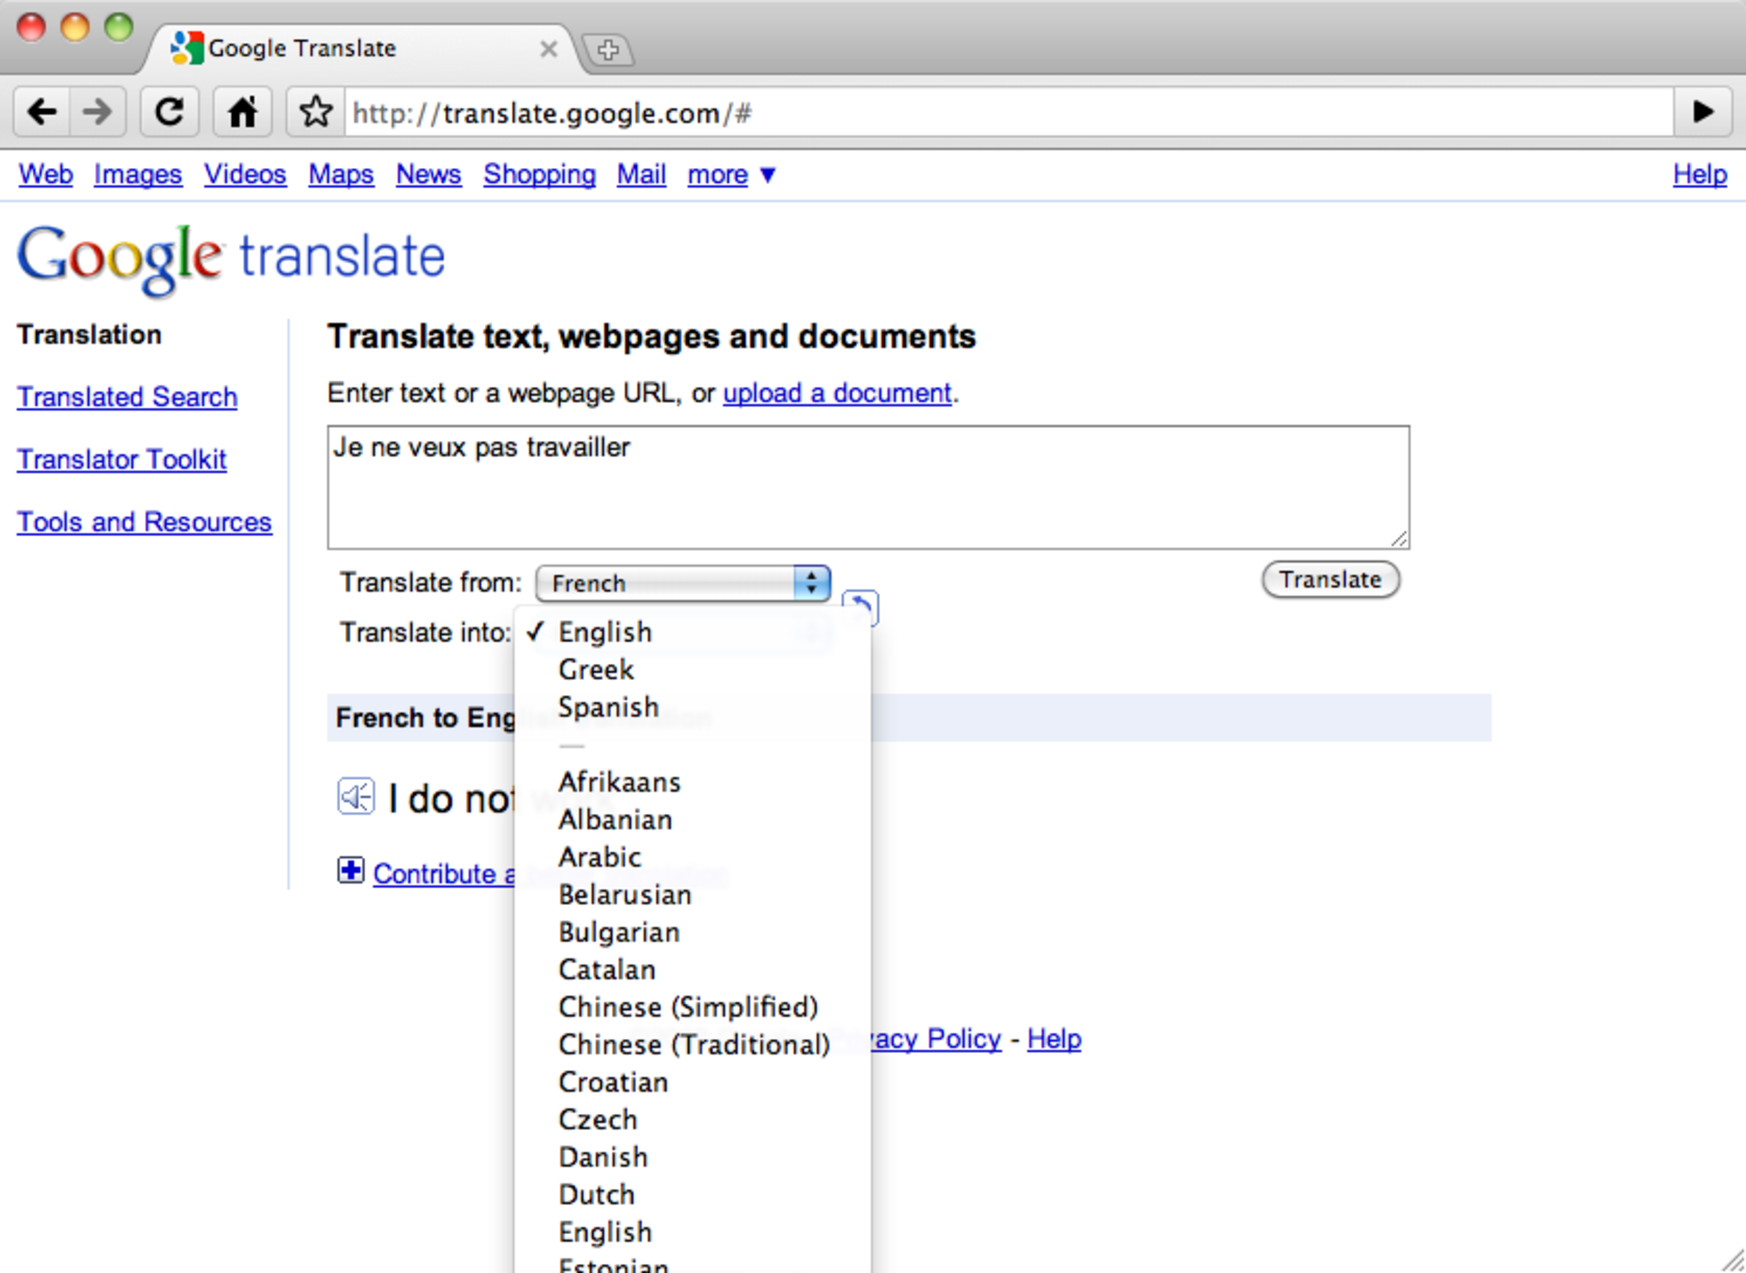
\includegraphics[scale=0.35]{GoogleTranslateLanguages.pdf}
\end{center}
\end{frame}

\begin{frame}[t]{Workshop overview}
Input:
  \begin{itemize}
%  \item Joshua decoder
  \item Existing procedures for synchronous grammar extraction
  \end{itemize}
\vspace{0.3in}
Output:
  \begin{itemize}
    \item New unsupervised models for large scale synchronous grammar extraction,
%    \item An implementation of this model,
    \item A comparison and analysis of the existing and proposed models,
    \item Extended decoders (cdec/Joshua) capable of working efficiently with these models.
  \end{itemize}
\end{frame}

\begin{frame}[t]{Models of translation}
\begin{exampleblock}{Supervised SCFG: Syntactic Tree-to-String}
\begin{center}
  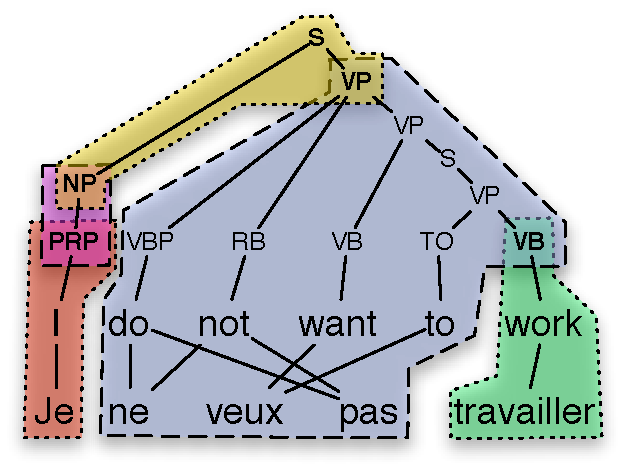
\includegraphics[scale=0.55]{JeNeVeuxPasTravailler-tsg.pdf}
  \hspace{0.3in}
  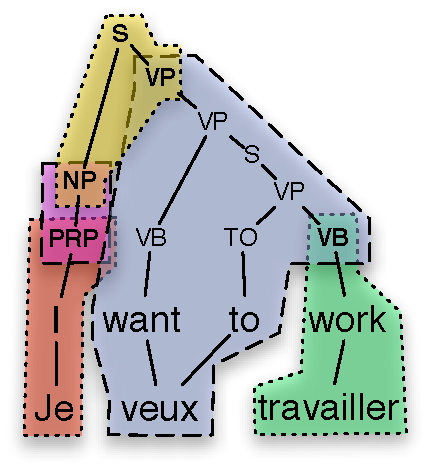
\includegraphics[scale=0.55]{JeVeuxTravailler-tsg.pdf}
\end{center}
\end{exampleblock}
\begin{itemize}
\item Strong model of sentence structure.
\item Reliant on a treebank to train the parser.
\end{itemize}
\end{frame}

\begin{frame}[t]{Models of translation}
\begin{block}{Unlabelled SCFG: Hiero}
  \begin{center}
    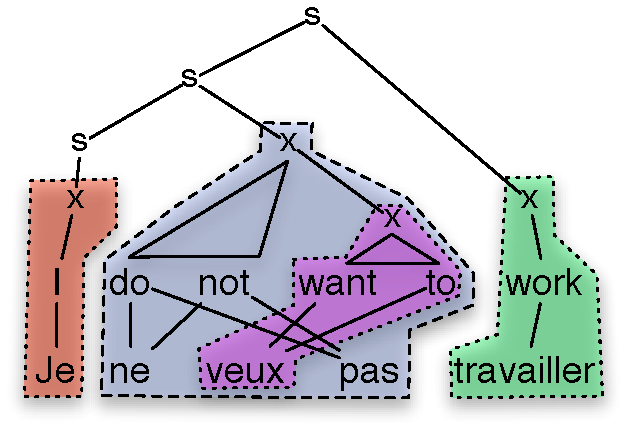
\includegraphics[scale=0.55]{JeNeVeuxPasTravailler-Hiero.pdf}
    \hspace{0.3in}
    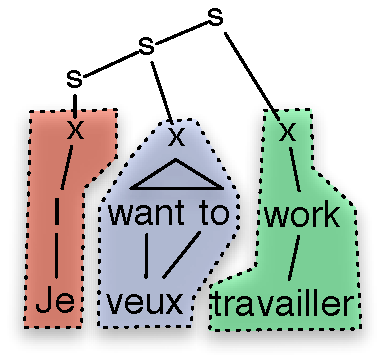
\includegraphics[scale=0.55]{JeVeuxTravailler-Hiero.pdf}
  \end{center}
\end{block}
\begin{itemize}
\item Only requires the parallel corpus.
\item But weak model of sentence structure.
\end{itemize}
\end{frame}

\begin{frame}
\frametitle{Using syntax in Machine Translation:}
  \footnotesize
  \begin{block}{Synchronous Context Free Grammar (SCFG)}
    \begin{figure}
    \begin{align*}
        \alert<2>{S} & \alert<2>{\rightarrow  \langle X\ind{1},\ X\ind{1} \rangle} 
            &\quad \alert<3,5>{X} & \alert<3,5>{\rightarrow  \langle X\ind{1}\ X\ind{2},\ X\ind{1}\ X\ind{2} \rangle} \\
        \alert<7>{X} & \alert<7>{\rightarrow  \langle X\ind{1}\ X\ind{2},\ X\ind{2}\ X\ind{1} \rangle} & &\\
        \alert<4>{X} & \alert<4>{\rightarrow  \langle Sie,\ She \rangle} 
           &\quad \alert<6>{X} & \alert<6>{\rightarrow  \langle will,\ wants\ to \rangle} \\
         \alert<8>{X} & \alert<8>{\rightarrow  \langle eine\ Tasse\ Kaffee,\ a\ cup\ of\ coffee \rangle}
           &\quad \alert<9>{X} & \alert<9>{\rightarrow  \langle trinken,\ drink\rangle} \\
    \end{align*}
    \end{figure}
  \end{block}
  \begin{exampleblock}{Example Derivation}
      %\begin{figure}
      %\begin{align*}
      \center
        \vspace{0.2cm}
        \onslide<2->{\alert<2>{$S \Rightarrow \langle X\ind{1},\ X\ind{1}\ \rangle$}} \quad \onslide<3->{\alert<3>{$\Rightarrow \langle X\ind{2}\ X\ind{3},\ X\ind{2}\ X\ind{3} \rangle$ \\}}
        \vspace{0.2cm}
        \onslide<4->{\alert<4>{$\Rightarrow \langle Sie\ X\ind{3},\ She\ X\ind{3} \rangle$}} \quad \onslide<5->{\alert<5>{$\Rightarrow \langle Sie\ X\ind{4}\ X\ind{5},\ She\ X\ind{4}\ X\ind{5} \rangle$ \\}}
        \vspace{0.2cm}
        \onslide<6->{\alert<6>{$\Rightarrow \langle Sie\ will\ X\ind{5},\ She\ wants\ to\  X\ind{5} \rangle$ }} \quad \onslide<7->{\alert<7>{$\Rightarrow \langle Sie\ will\ X\ind{6} X\ind{7},\ She\ wants\ to\  X\ind{7} X\ind{6} \rangle$ \\}}
        \vspace{0.2cm}
        \onslide<8->{\alert<8>{$\Rightarrow \langle Sie\ will\ eine\ Tasse\ Kaffee\ X\ind{7},\ She\ wants\ to\ X\ind{7}\ a\ cup\ of\ coffee\rangle$} \\}
        \vspace{0.2cm}
        \onslide<9->{\alert<9>{$\Rightarrow \langle Sie\ will\ eine\ Tasse\ Kaffee\ trinken,\ She\ wants\ to\ drink\ a\ cup\ of\ coffee\rangle$}}
        \vspace{0.2cm}
      %\end{align*}
      %\end{figure}
  \end{exampleblock}
\end{frame}

\begin{frame}[t]{Models of translation}
\begin{exampleblock}{Phrase extraction:}
\begin{center}
\only<1>{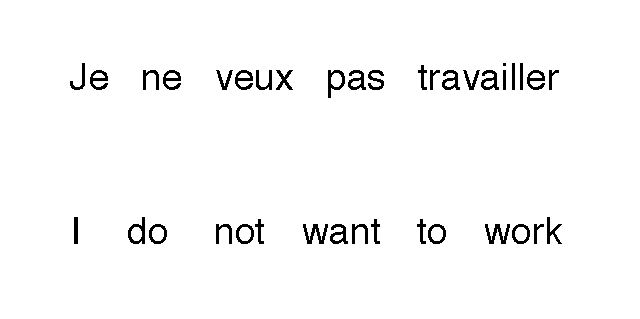
\includegraphics[scale=0.8]{PhraseExtraction6.pdf}\\[1cm]}
\only<2>{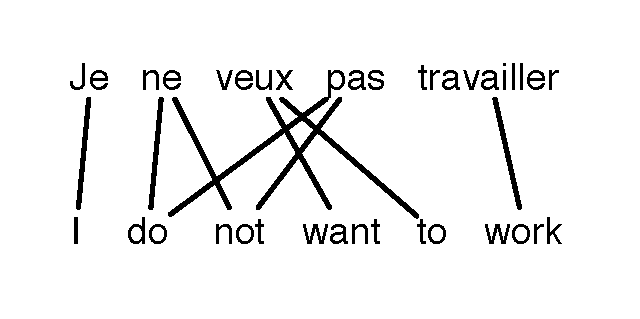
\includegraphics[scale=0.8]{PhraseExtraction5.pdf}\\[1cm]}
\only<3>{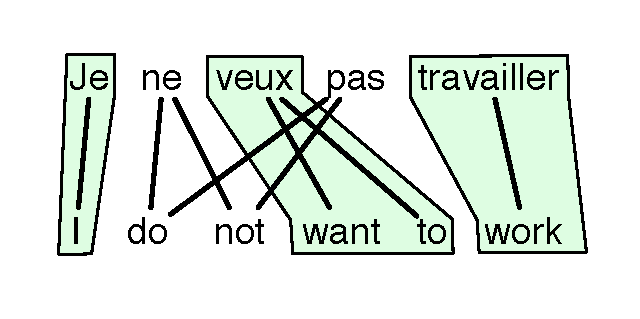
\includegraphics[scale=0.8]{PhraseExtraction4.pdf}\\[1cm]}
\only<4>{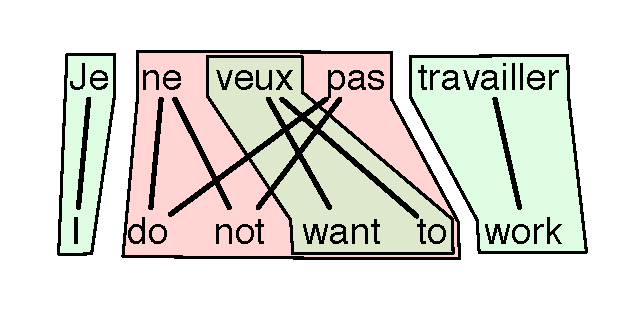
\includegraphics[scale=0.8]{PhraseExtraction3.pdf}\\[1cm]}
\only<5>{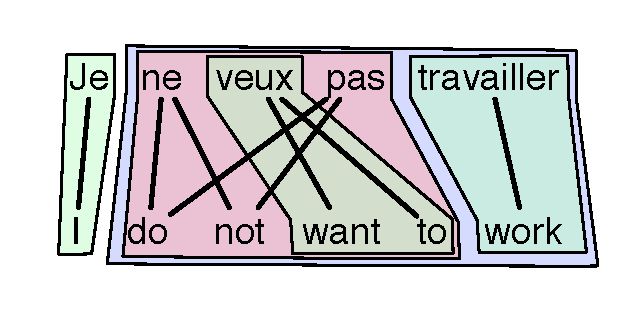
\includegraphics[scale=0.8]{PhraseExtraction2.pdf}\\[1cm]}
\only<6>{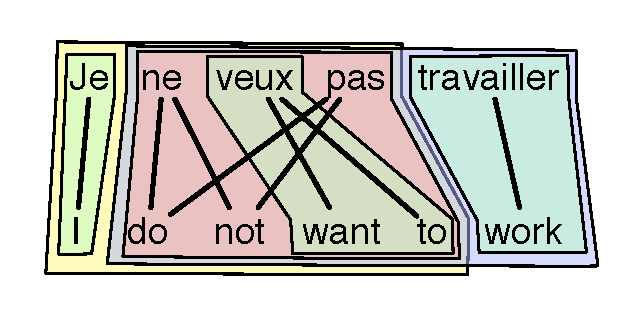
\includegraphics[scale=0.8]{PhraseExtraction1.pdf}\\[1cm]}
\only<7>{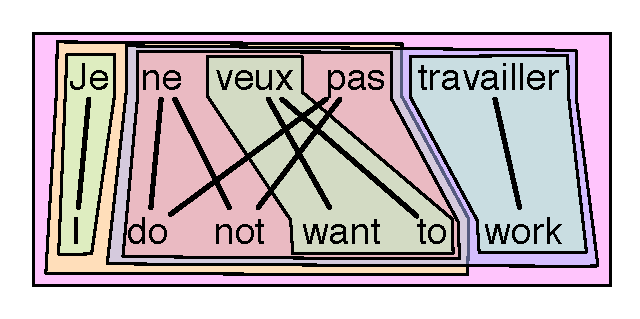
\includegraphics[scale=0.8]{PhraseExtraction.pdf}\\[1cm]}
\end{center}
\end{exampleblock}
\only<2->{
\begin{unpacked_itemize}
\only<2>{\item Use a word-based translation model to annotate the parallel corpus with word-alignments}
\only<3->{\item $\langle$ Je, I $\rangle$, $\langle$ veux, want to $\rangle$,  $\langle$ travailler, work $\rangle$}\only<4->{, $\langle$ ne veux pas, do not want to $\rangle$}\only<5->{, $\langle$ ne veux pas travailler, do not want to work $\rangle$}\only<6->{, $\langle$ Je ne veux pas, I do not want to $\rangle$}\only<7->{, $\langle$ Je ne veux pas travailler, I do not want to work $\rangle$}
\end{unpacked_itemize}
}
\end{frame}


\begin{frame}[t]{Models of translation}
\begin{exampleblock}{SCFG Rule extraction:}
\begin{center}
\only<1>{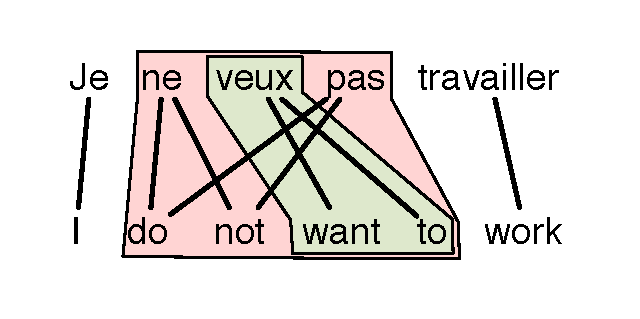
\includegraphics[scale=0.8]{HieroExtraction1.pdf}\\[1cm]}
\only<2>{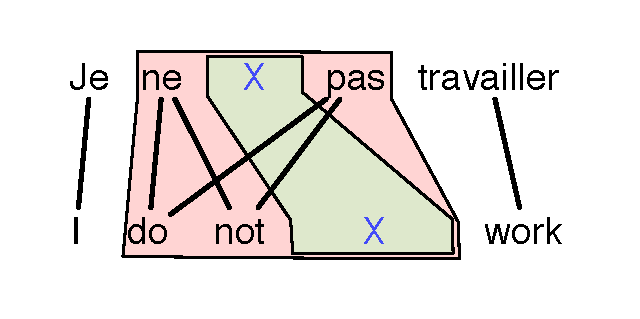
\includegraphics[scale=0.8]{HieroExtraction2.pdf}\\[1cm]}
\only<3>{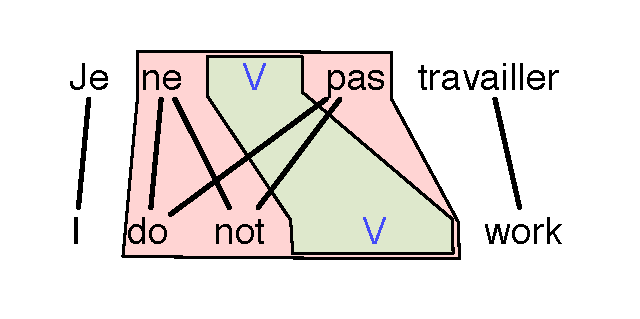
\includegraphics[scale=0.8]{HieroExtraction3.pdf}\\[1cm]}
\only<4>{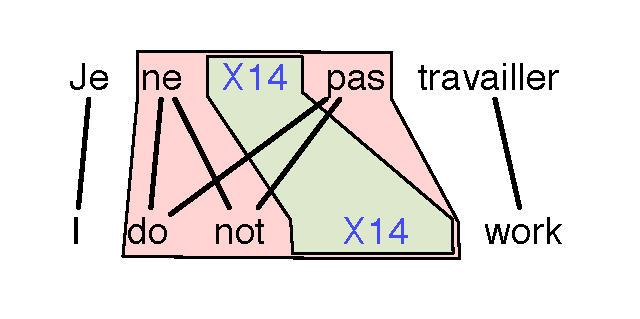
\includegraphics[scale=0.8]{HieroExtraction4.pdf}\\[1cm]}
\end{center}
\end{exampleblock}
\begin{unpacked_itemize}
\only<1>{ \item X -> $\langle$ ne veux pas, do not want to $\rangle$ }
\only<2>{ \item X -> $\langle$ ne veux pas, do not want to $\rangle$, \item X -> $\langle$ ne X\ind{1} pas, do not X\ind{1} $\rangle$ }
\only<3>{ \item VP$/$NN -> $\langle$ ne veux pas, do not want to $\rangle$, \item VP$/$NN -> $\langle$ ne V\ind{1} pas, do not V\ind{1} $\rangle$ }
\only<4>{ \item X10 -> $\langle$ ne veux pas, do not want to $\rangle$, \item X10 -> $\langle$ ne X14\ind{1} pas, do not X14\ind{1} $\rangle$ }
\end{unpacked_itemize}
\end{frame}

%\begin{frame}[t]{Models of translation}
%\begin{block}{Hierarchical}
%  \begin{center}
%    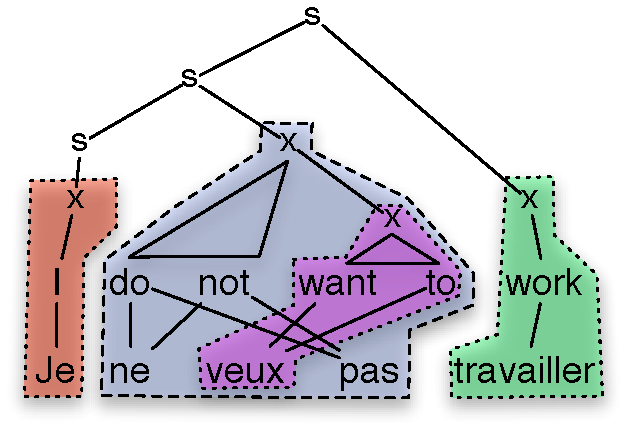
\includegraphics[scale=0.55]{JeNeVeuxPasTravailler-Hiero.pdf}
%    \hspace{0.3in}
%    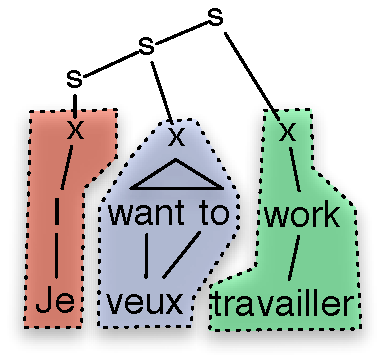
\includegraphics[scale=0.55]{JeVeuxTravailler-Hiero.pdf}
%  \end{center}
%\end{block}
%\end{frame}


%\begin{frame}[t]{Impact}
%  \begin{center}
%    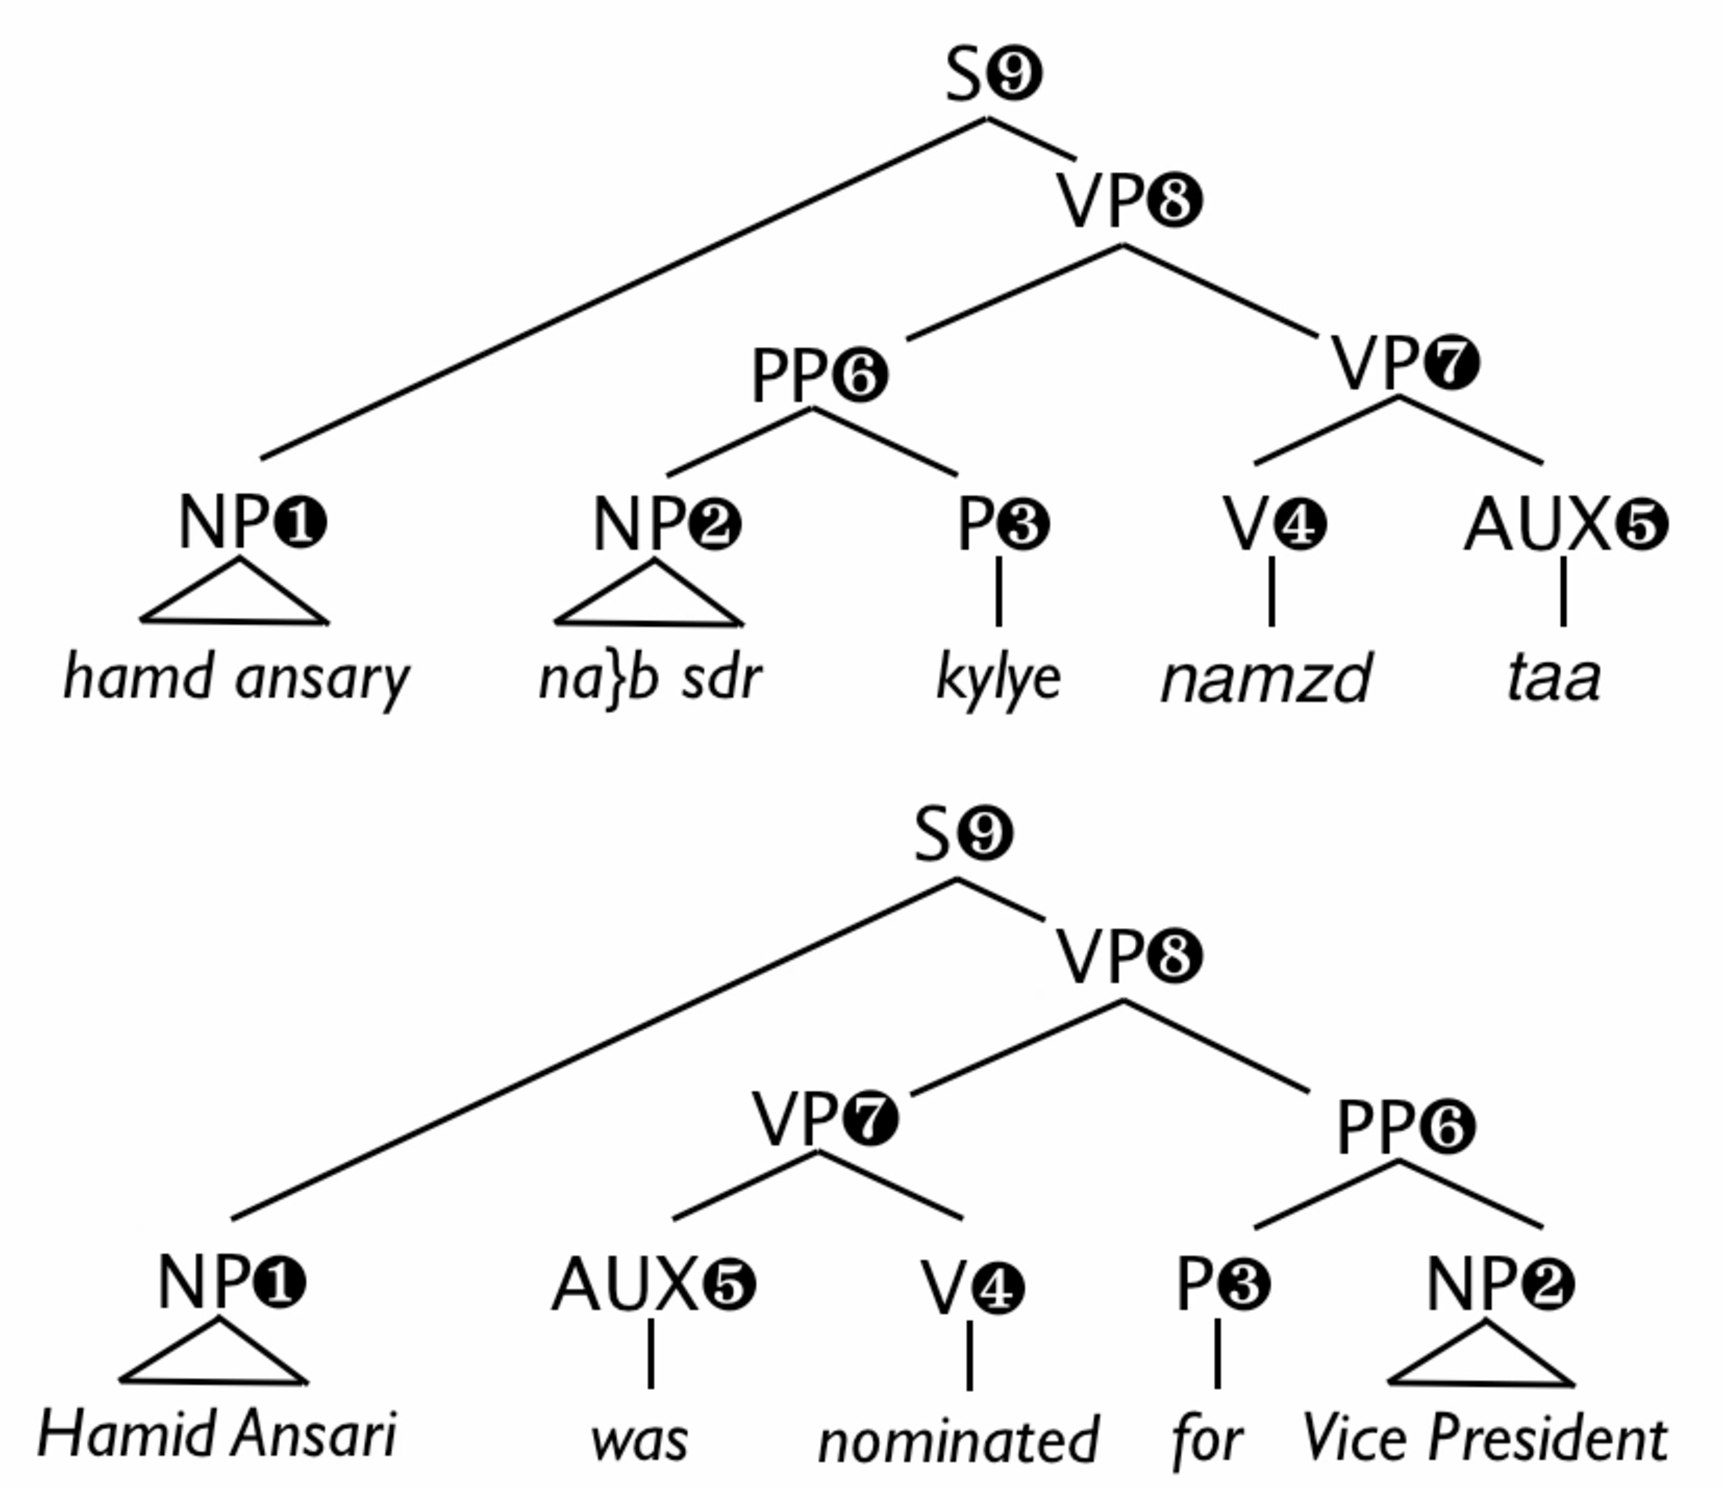
\includegraphics[scale=0.3]{ccb_tree.pdf}
%  \end{center}
%\end{frame}


\begin{frame}[t]{Impact}
\vspace{0.5in}
\begin{table}
  \begin{tabular}{l|rr}
    \hline
    Language & Words &  Domain \\ \hline
    English & 4.5M& Financial news \\
    Chinese & 0.5M & Broadcasting news \\ 
    Arabic &  300K (1M planned)  &  News  \\
    Korean & 54K  & Military \\ \hline
  \end{tabular}
\caption{Major treebanks: data size and domain \label{table_treebanks_size}}
\end{table}
\end{frame}


\begin{frame}[t]{Impact}
Parallel corpora far exceed treebanks (millions of words):
  \begin{figure}
    {\centering 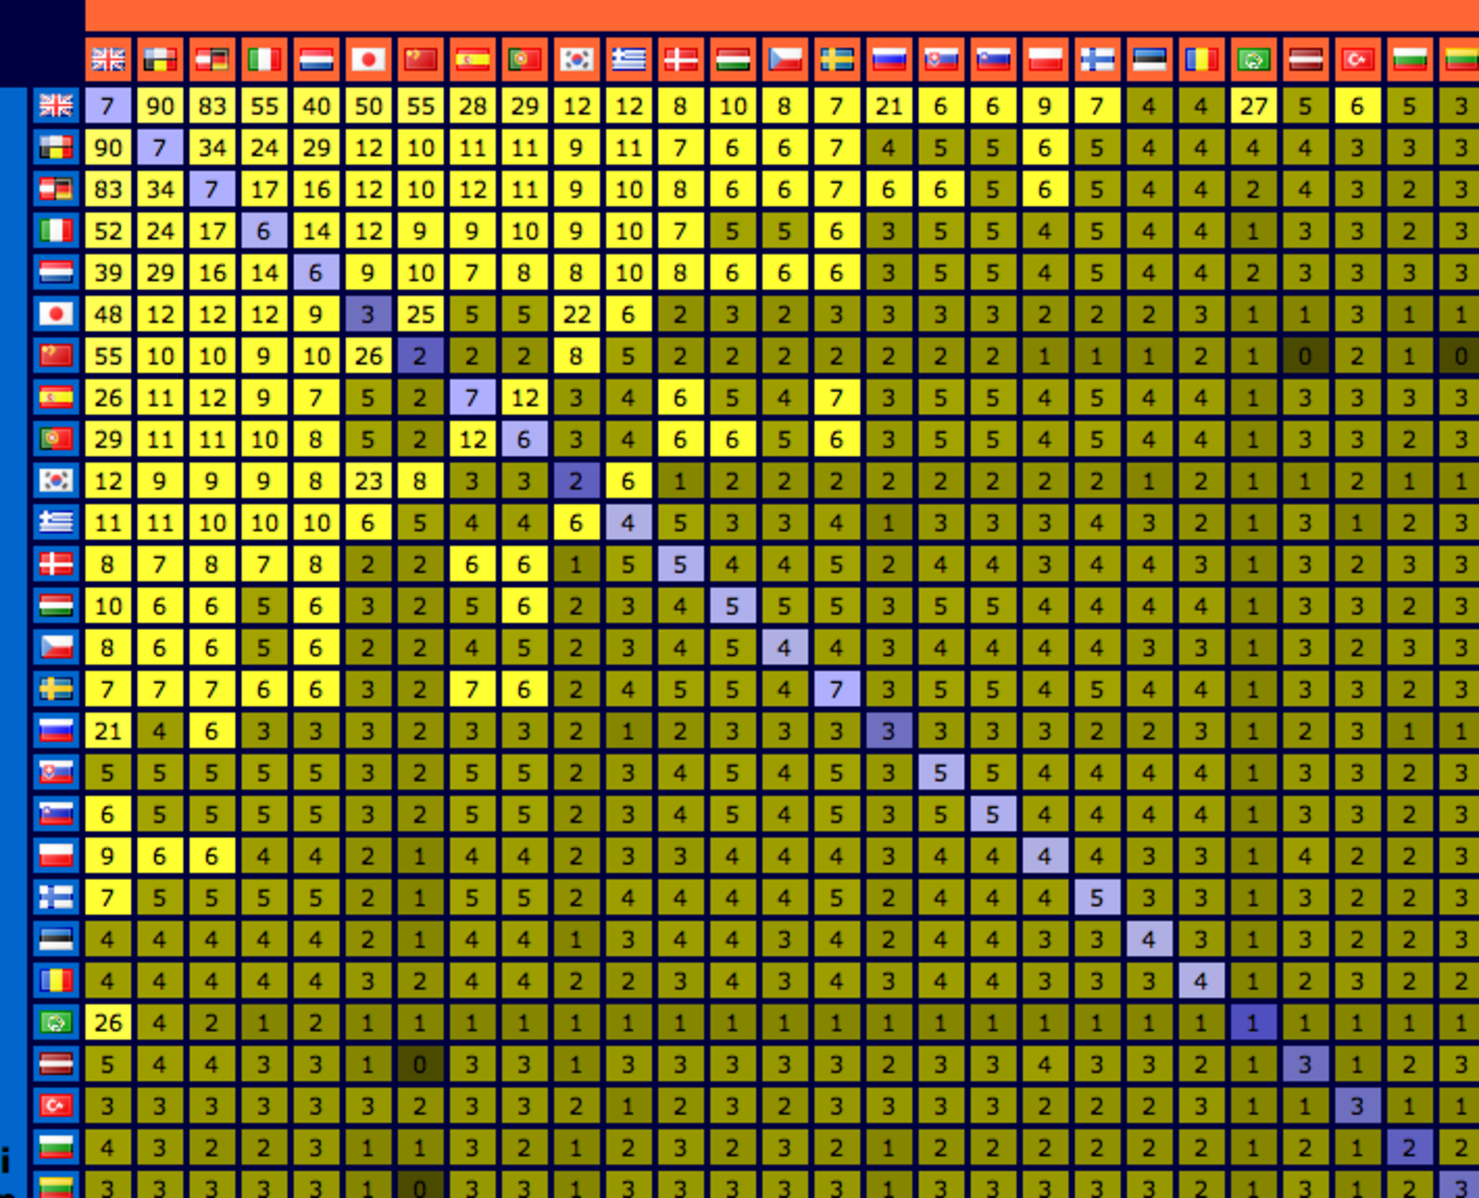
\includegraphics[scale=0.7]{resource_matrix.pdf}}
  \end{figure}
\end{frame}


\begin{frame}[t]{Models of translation}
\begin{block}{Hierarchical}
  \begin{center}
    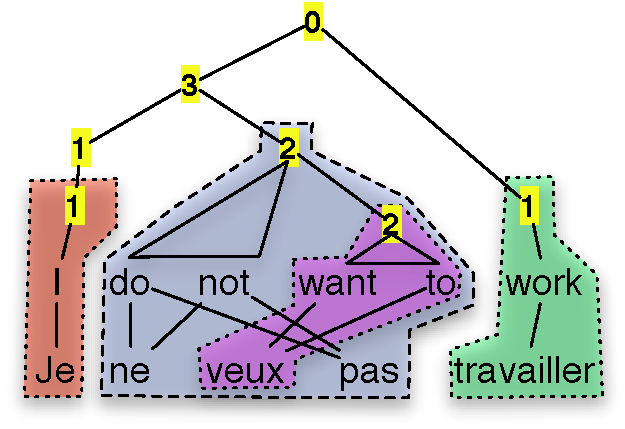
\includegraphics[scale=0.55]{JeNeVeuxPasTravailler-Hiero-labelled.pdf}
    \hspace{0.3in}
    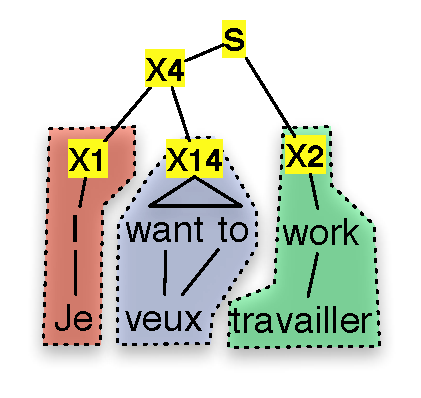
\includegraphics[scale=0.55]{JeVeuxTravailler-Hiero-labelled.pdf}
  \end{center}
\end{block}
\begin{itemize}
\item \alert{AIM: Implement a large scale open-source synchronous constituent learning system.} 
\item \alert{AIM: Investigate and understand the relationship between the choice of synchronous grammar and SMT performance,} 
\item \alert{AIM: and fix our decoders accordingly.} 
\end{itemize}
\end{frame}

\begin{frame}[t]{Evaluation goals}
We will predominately evaluate using BLEU, but also use automatic structured metrics and perform small scale human evaluation:
\vspace{0.25in}
\begin{unpacked_itemize}
\item Evaluate phrasal, syntactic, unsupervised syntactic,
\item Aim 1: Do no harm (not true of existing syntactic approach)
\item Aim 2: Exceed the performance of current non-syntactic systems.
\item Aim 3: Meet or exceed performance of existing syntactic systems.
\end{unpacked_itemize}
\end{frame}

%\begin{frame}[t]{Impact}
%Success will have a significant impact on two areas of CL:
%\vspace{0.25in}
%\begin{unpacked_itemize}
%\item Machine translation
%\begin{unpacked_itemize}
%  \item Make the benefits of richly structured translation models available to a much wider range of researchers and for a wider range of languages.
%% \item Change the research outlook of the field.
%\end{unpacked_itemize}
%\item Grammar induction:
%\begin{unpacked_itemize}
%  \item Provide an empirical validation of state-of-the-art grammar induction techniques.
%\end{unpacked_itemize}
%\end{unpacked_itemize}
%\end{frame}


\begin{frame}[t]{Workshop Streams}
\vspace{0.25in}
\begin{unpacked_itemize}
\item Implement scalable SCFG grammar extraction algorithms.
\item Improve SCFG decoders to effieciently handle the grammars produce.
\item Investigate discriminative training regimes the leverage features extracted from these grammars.
\end{unpacked_itemize}
\end{frame}


%\begin{frame}[t]
%\frametitle{Inducing a STSG given an observed tree:}
%\only<1>{\frametitle{Inducing a STSG given an observed tree:}}
%\only<2->{\frametitle{Existing approach (Galley et al. 2004):}}
%
%\begin{center}
%  \only<1>{\hspace{1mm}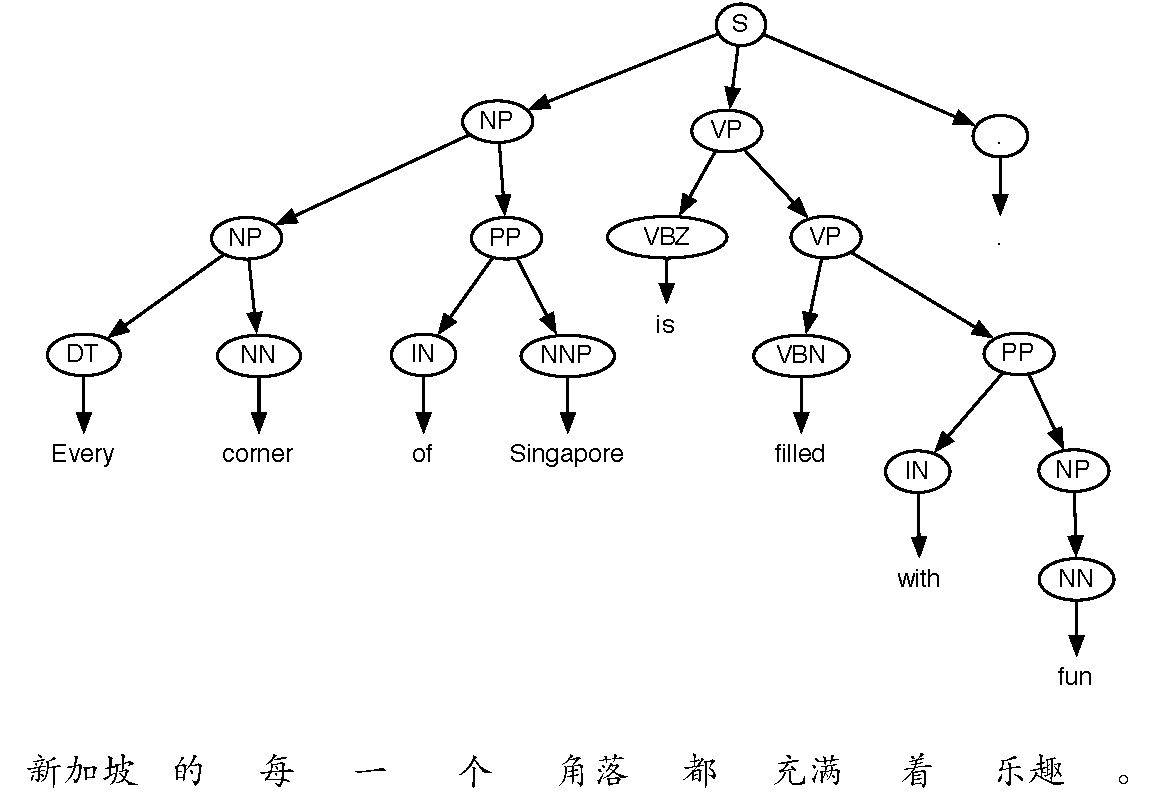
\includegraphics[scale=0.45]{full_of_fun_slides_start.pdf}}
%  \only<2>{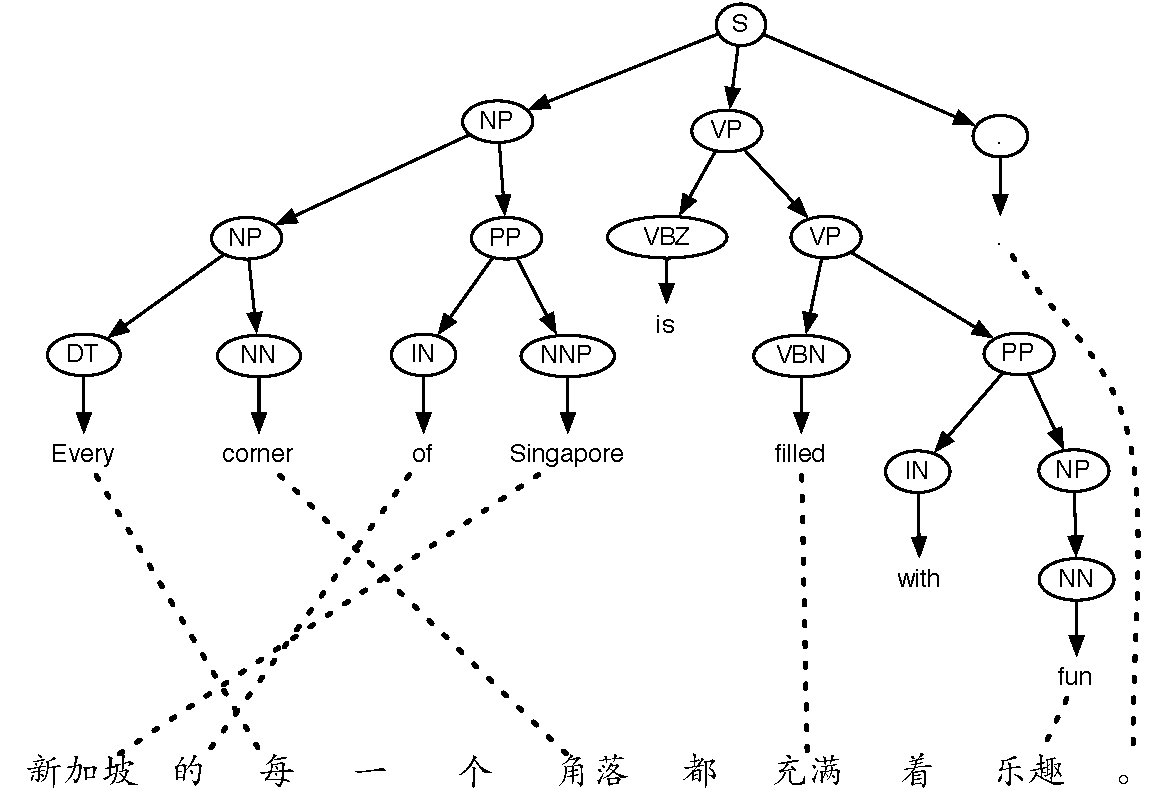
\includegraphics[scale=0.45]{full_of_fun_slides_waligned.pdf}}
%  \only<3>{\vspace{-2mm}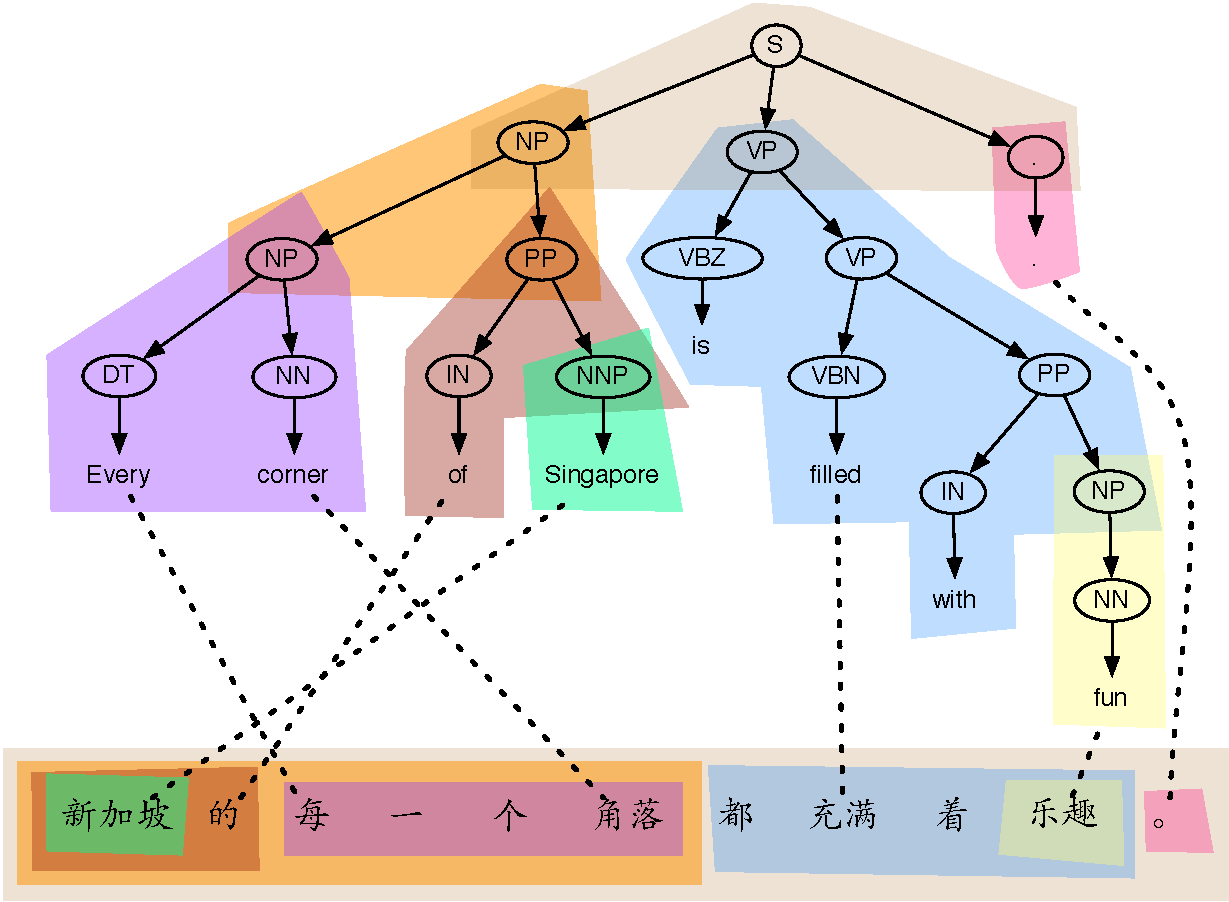
\includegraphics[scale=0.45]{full_of_fun_slides_waligned_overlay.pdf}}
%% \only<4>{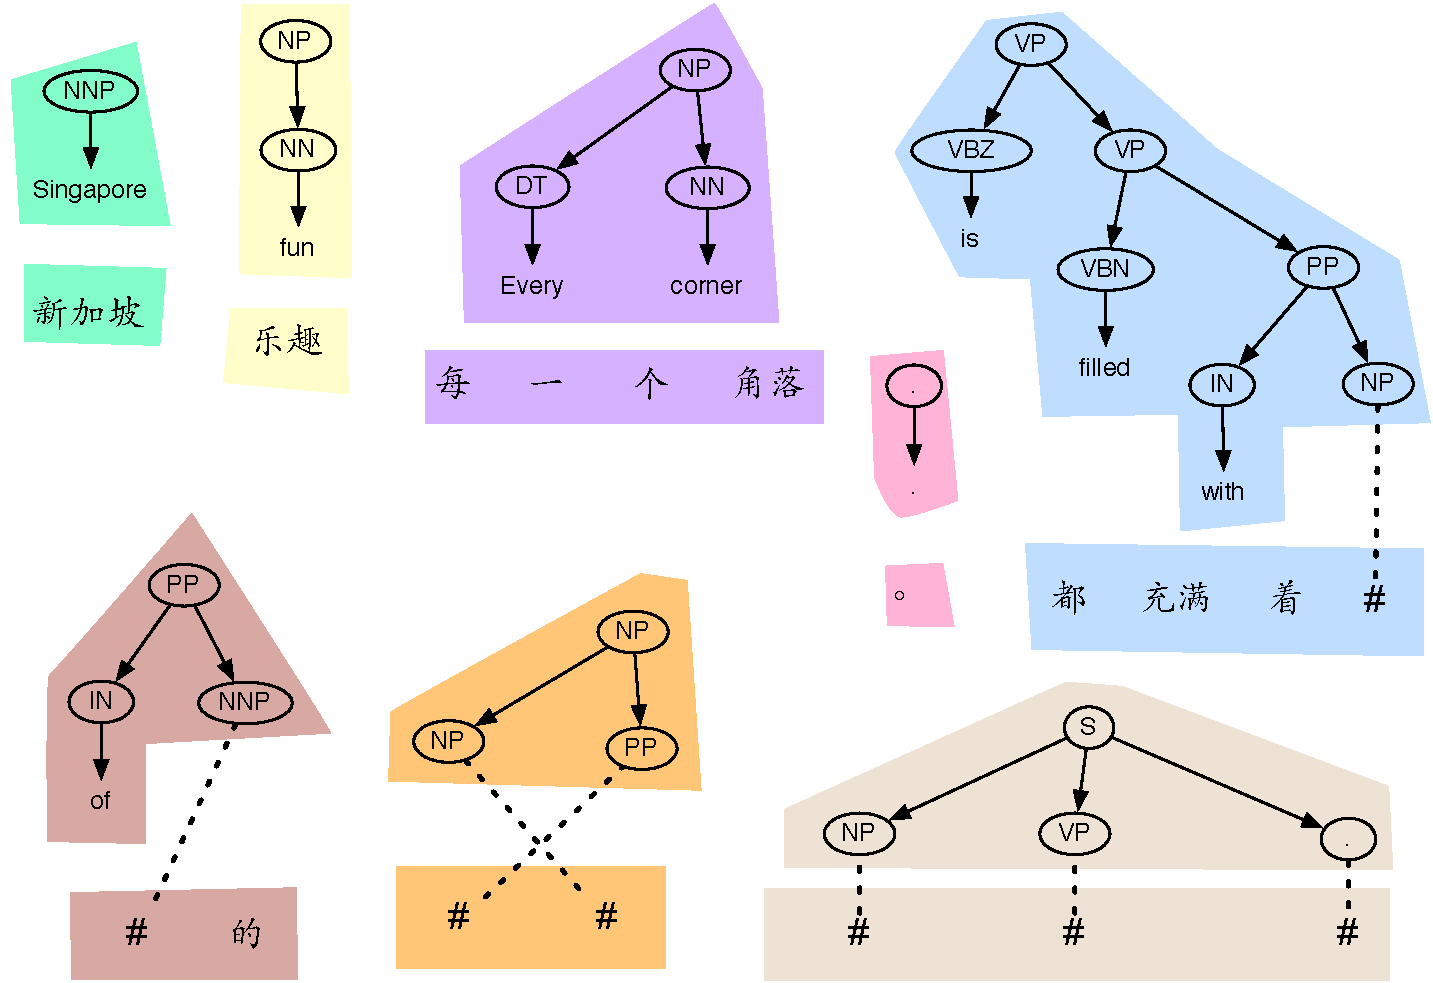
\includegraphics[scale=0.4]{full_of_fun_slides_third.pdf}}
%% \only<5>{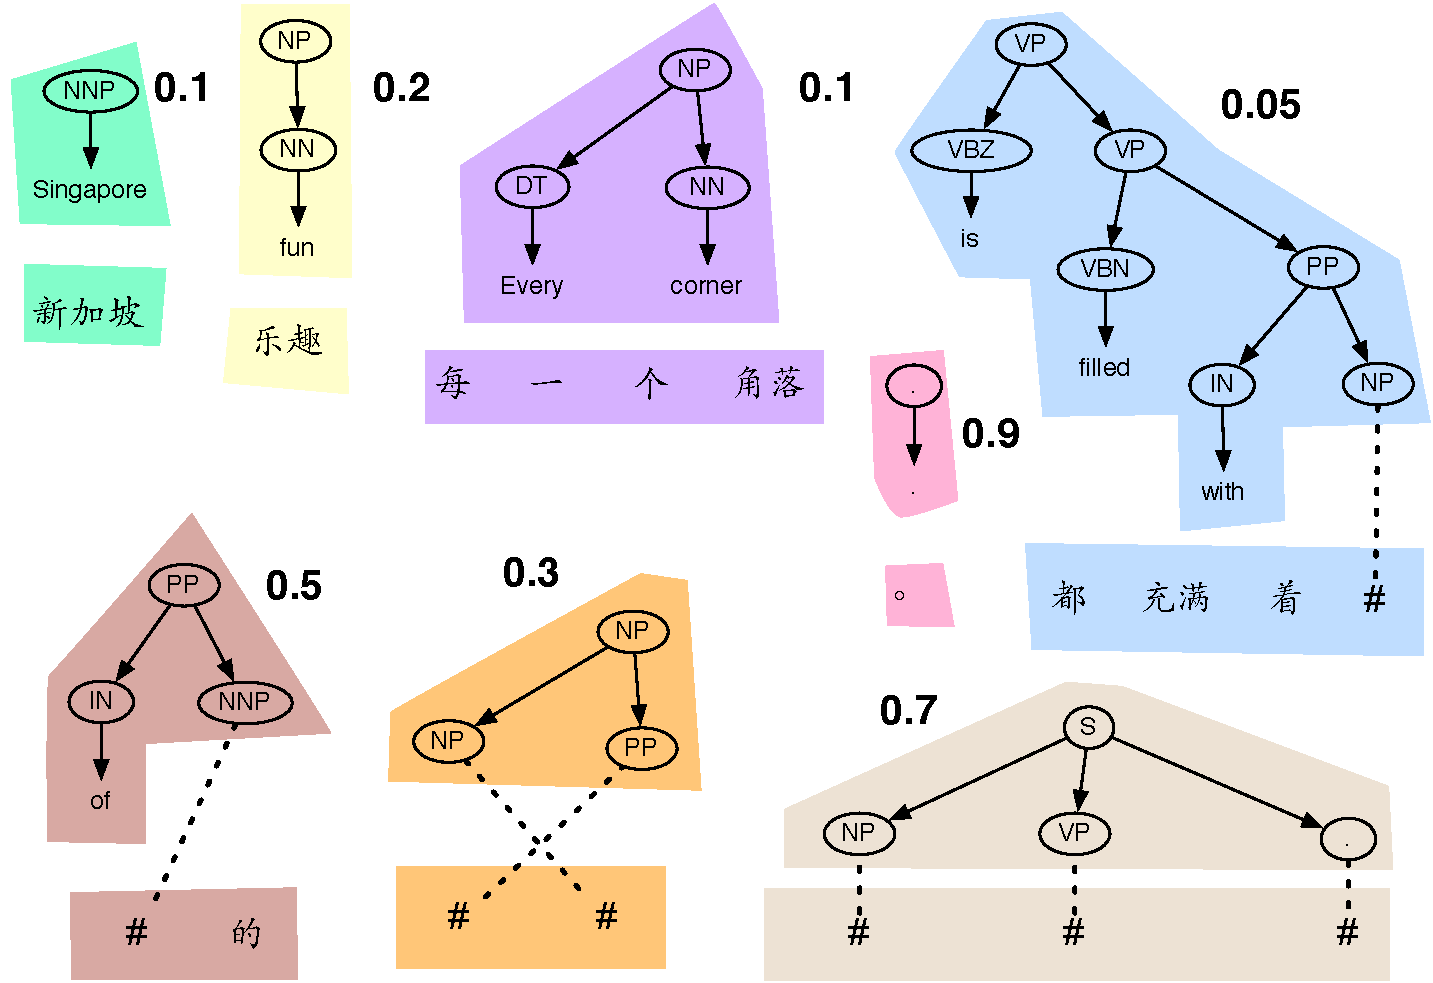
\includegraphics[scale=0.4]{full_of_fun_slides_forth.pdf}}  
%
%  \only<1>{Training instance}
%  \only<2>{Step 1: word alignment}
%  \only<3>{Step 2: rule extraction heuristic}
%% \only<4>{Step 2: the rules extracted}
%% \only<5>{Step 3: estimate a grammar}
%\end{center}
%\end{frame}


% Il ne veut pas travailler


%\begin{frame}[t]{Models of translation}
%\begin{block}{Hierarchical}
%  \begin{center}
%    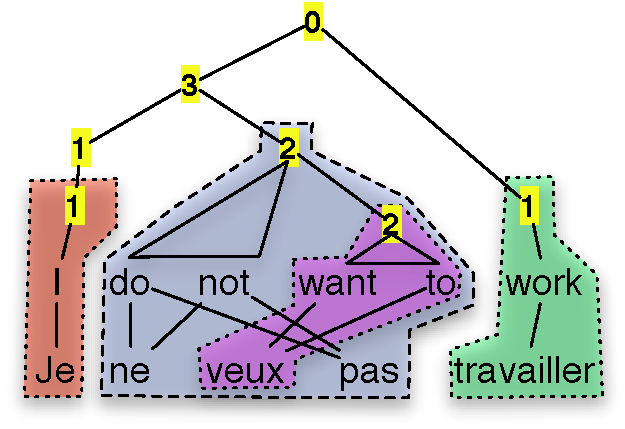
\includegraphics[scale=0.55]{JeNeVeuxPasTravailler-Hiero-labelled.pdf}
%    \hspace{0.3in}
%    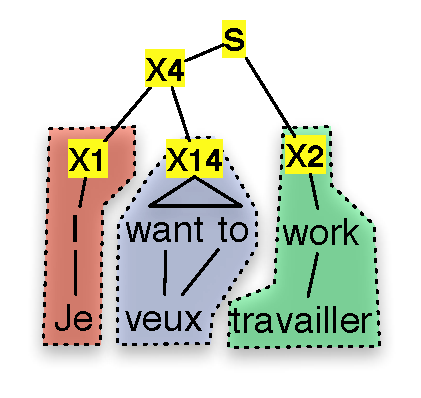
\includegraphics[scale=0.55]{JeVeuxTravailler-Hiero-labelled.pdf}
%  \end{center}
%\end{block}
%\begin{itemize}
%\item \alert{AIM: Implement a large scale open-source synchronous constituent labelling system.} 
%\item \alert{AIM: Investigate and understand the relationship between synchronous constituency and SMT performance.} 
%\end{itemize}
%\end{frame}
%
%\begin{frame}[t]{Models of translation}
%\begin{block}{Hierarchical}
%  \begin{center}
%    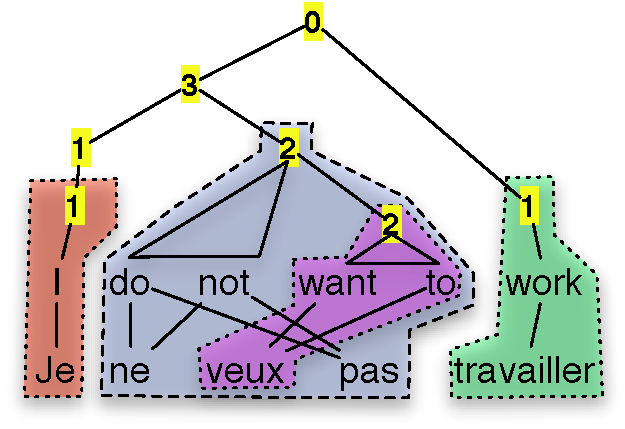
\includegraphics[scale=0.5]{JeNeVeuxPasTravailler-Hiero-labelled.pdf}
%    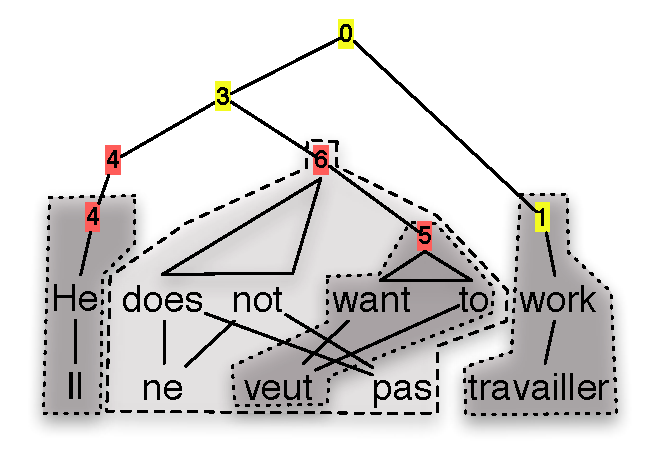
\includegraphics[scale=0.5]{IlNeVeutPasTravailler-Hiero-labelled.pdf}
%  \end{center}
%  \vspace{0.001in}
%\end{block}
%\begin{itemize}
%\item \alert{AIM: Implement a large scale open-source synchronous constituent labelling system.} 
%\item \alert{AIM: Investigate and understand the relationship between synchronous constituency and SMT performance.} 
%\end{itemize}
%\end{frame}

\begin{frame}[t]{Unsupervised grammar induction}
There has been significant research into monolingual grammar induction:
\vspace{0.1in}
\alert{Constituent context is a prime indicator of constituency.}
\begin{unpacked_itemize}
\item Alexander Clark. Unsupervised induction of stochastic context-free grammars using distributional clustering, 2001
\item Dan Klein and Chris Manning. A Generative Constituent-Context Model for Improved Grammar Induction, 2002
\end{unpacked_itemize}
\vspace{0.1in}
\alert{We can formalise this notion in algebraic structures}
\begin{itemize}
\item Alexander Clark. A learnable representation for syntax using residuated lattices, 2009
\end{itemize}
\vspace{0.1in}
Deep connections to unsupervised word sense disambiguation, thesaurus extraction etc.
\end{frame}

%\begin{frame}[t]{Monolingual grammar induction}
%Induce bracketing phrase-structure grammars:
%  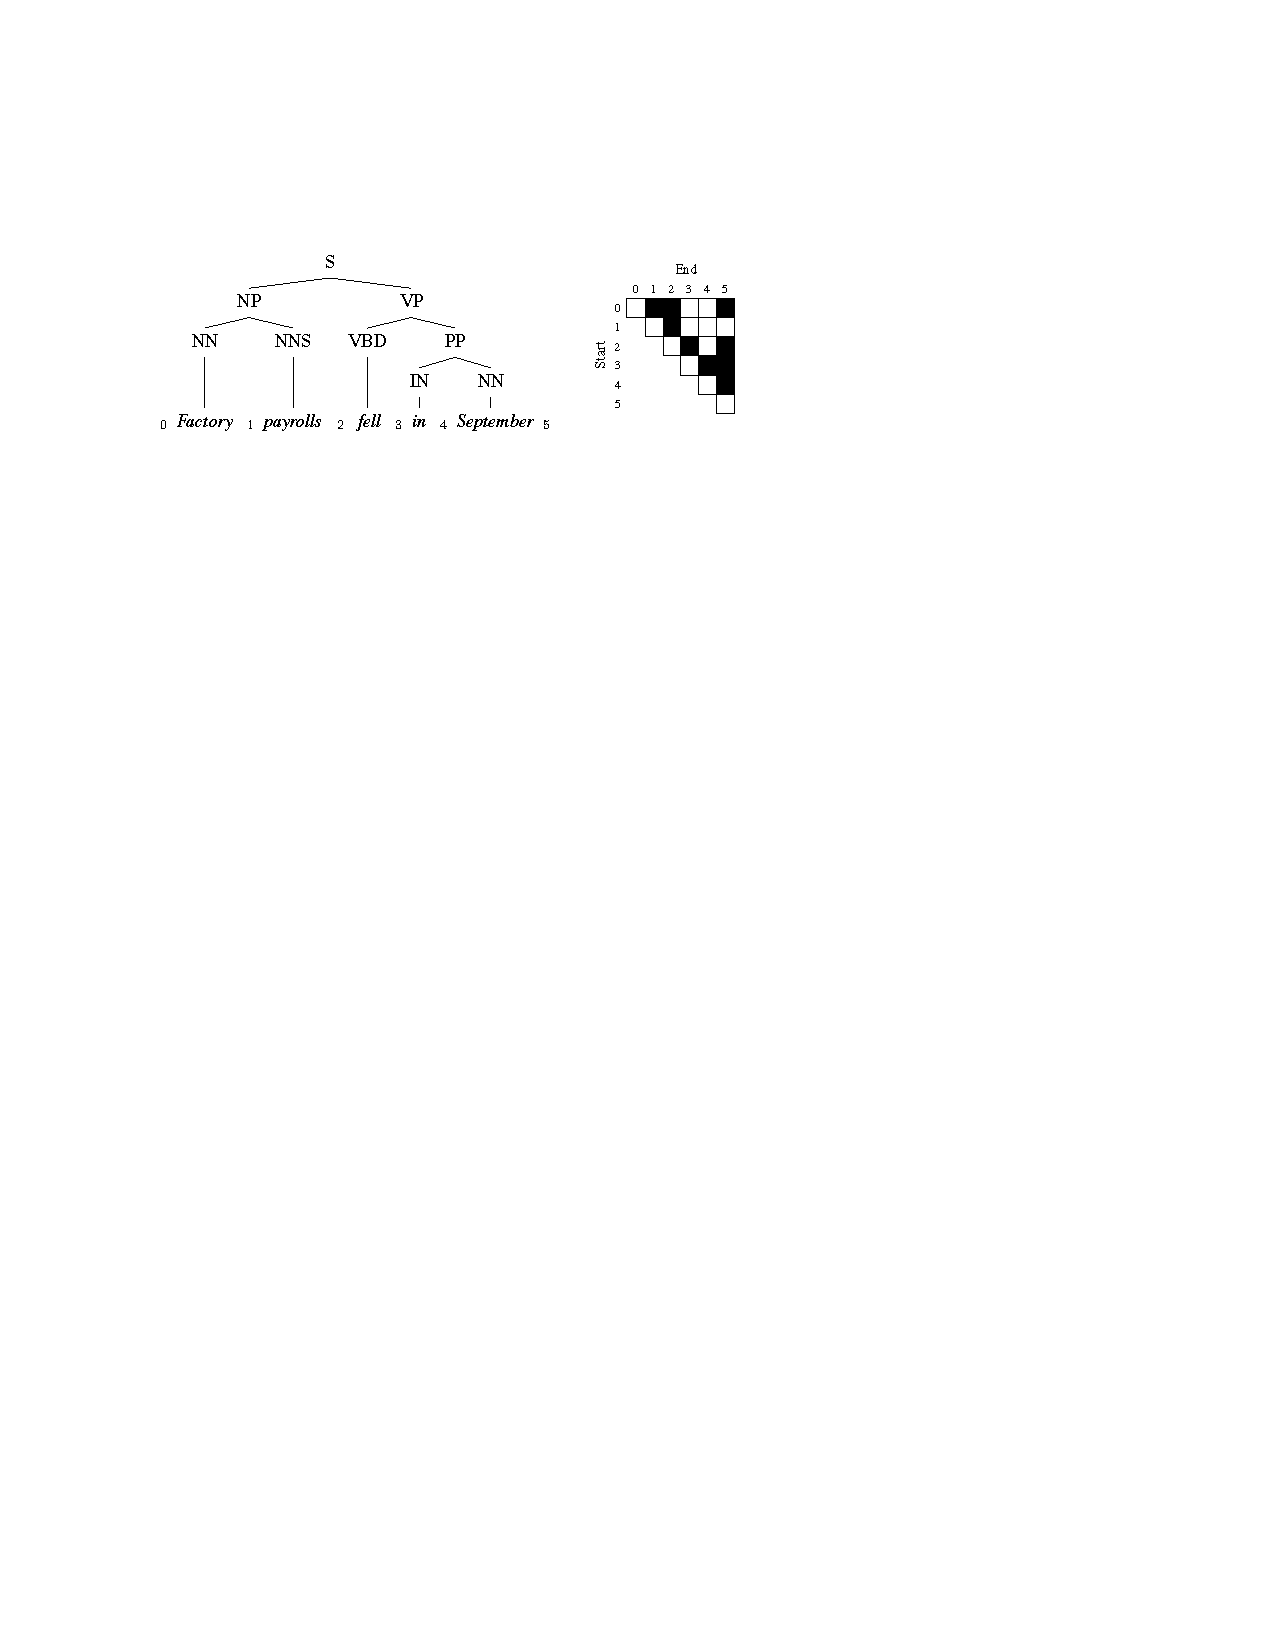
\includegraphics[scale=1]{klein_ccm.pdf} 
%
%\vspace{2ex}
%And dependency trees: \\
%  
\includegraphics[scale=1]{klein_dependency.pdf}
%
%\vspace{2ex}
%Informed by constituent context: surrounding words are a good indicator of substitutability
%\end{frame}


\begin{frame}[t]{SCFG Grammar Induction}
%\vspace{1.0cm}
\begin{exampleblock}{Distributional Hypothesis}
\begin{quote}
\emph{Words that occur in the same contexts tend to have similar meanings}
\end{quote}
\hfill (Zellig Harris, 1954)
\end{exampleblock}

\vspace{3ex}

We will leverage this in a translation setting:
\begin{itemize}
    \item Use the contexts to \alert{cluster} translation units into groups
    \item Units in the same group expected to be semantically and syntactically similar
    \item Then use these cluster labels to guide translation
    \begin{itemize}
        \item lexical selection: translating ambiguous source word/s
        \item reordering: consistent syntactic patterns of reordering
    \end{itemize}
\end{itemize}
\end{frame}

\begin{frame}[t]{Monolingual Example}
Task: cluster words into their parts-of-speech. \\

\vspace{1ex}
Illustrate by starting with the word `deal' (noun or verb):

\only<1>{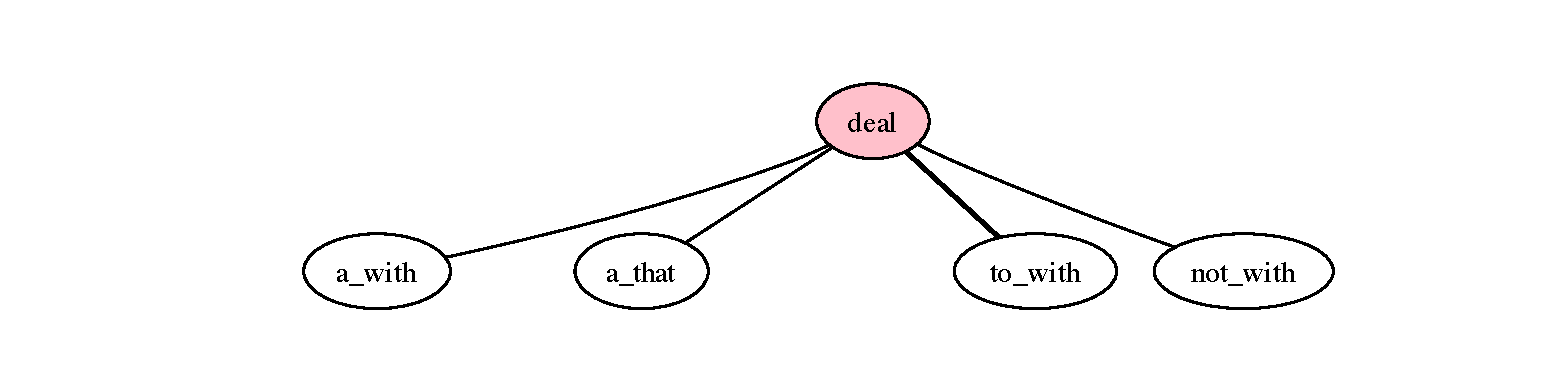
\includegraphics[width=\columnwidth]{deal_first.pdf} \\ Step 1: Find contexts for `deal'}
\only<2->{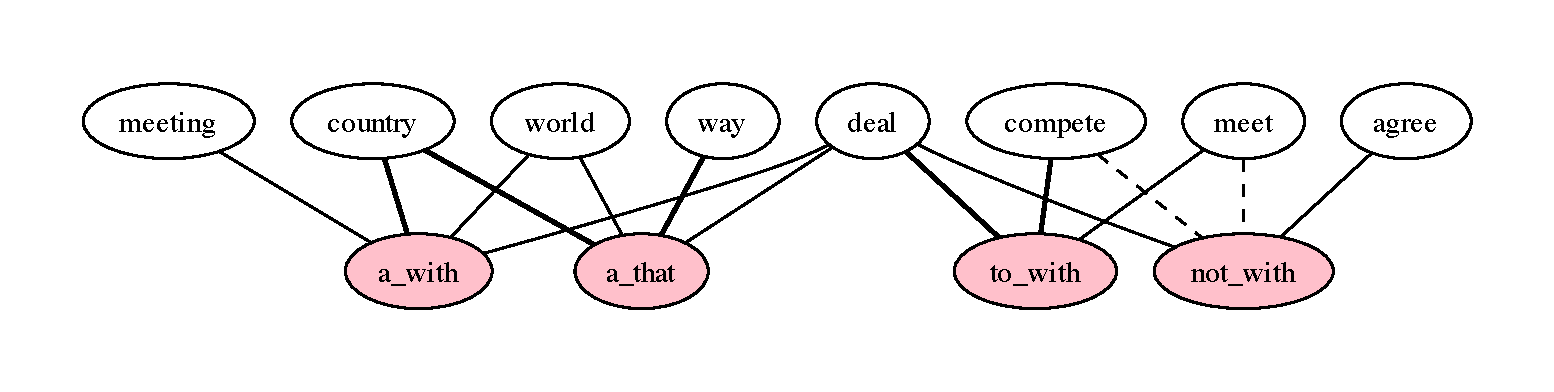
\includegraphics[width=\columnwidth]{deal.pdf} \\ Step 2: Find other words which occur in these contexts}
%\only<3>{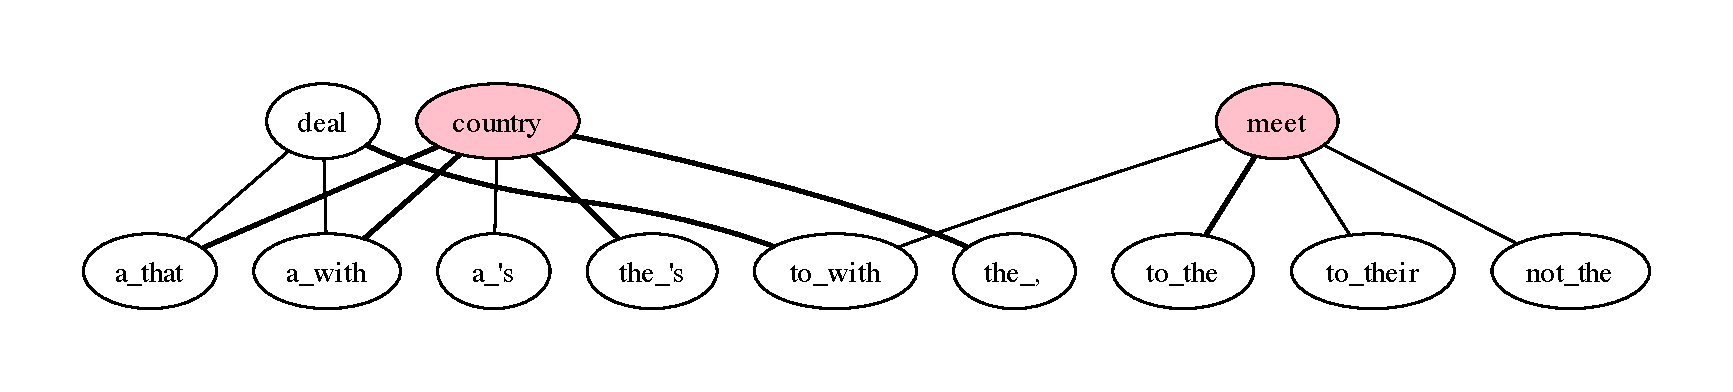
\includegraphics[width=\columnwidth]{deal_more.pdf} \\ \ldots continue to expand}

\only<3>{
\vspace{1ex}
Notice that the instances of deal can be split into two connected sub-graphs:
\begin{itemize}
    \item noun: the left two contexts ``a \ldots with'' and ``a \ldots that''
    \item verb: the right two contexts ``to \ldots with'' and ``not \ldots with''
    \item neighbouring words of these contexts share the same PoS
\end{itemize}
}

\end{frame}

%\begin{frame}[t]{More Formally}
%
%Construct a bipartite graph
%\begin{itemize}
%    \item Nodes on the top layer denote word types (bilingual phrase pairs)
%    \item Nodes on the bottom layer denote context types (monlingual/bilingual words)
%    \item Edges connect words and their contexts
%\end{itemize}
%
%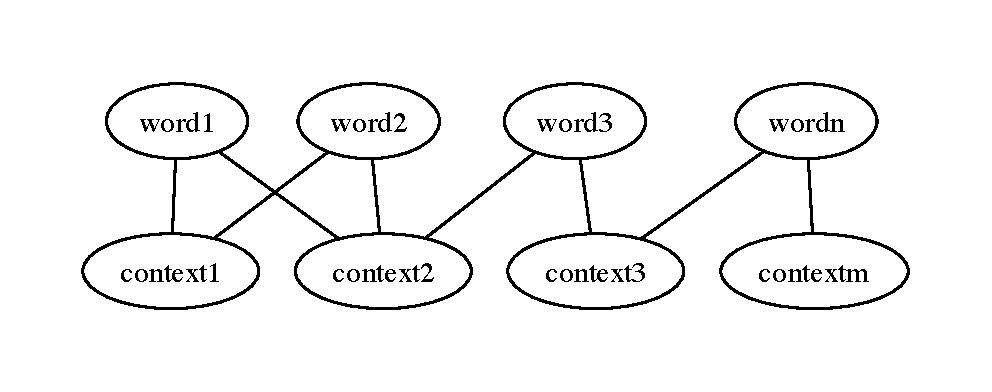
\includegraphics[width=\columnwidth]{bipartite.pdf}
%
%\end{frame}

\begin{frame}[t]{Clustering}

Task is to cluster the graph into sub-graphs. Nodes in the sub-graphs should be
\begin{itemize}
\item strongly connected to one another
\item weakly connected to nodes outside the sub-graph
\item could formulate as either \emph{hard} or \emph{soft} clustering
\end{itemize}
Choose \alert{soft clustering} to allow for syntactic and semantic ambiguity

\centering
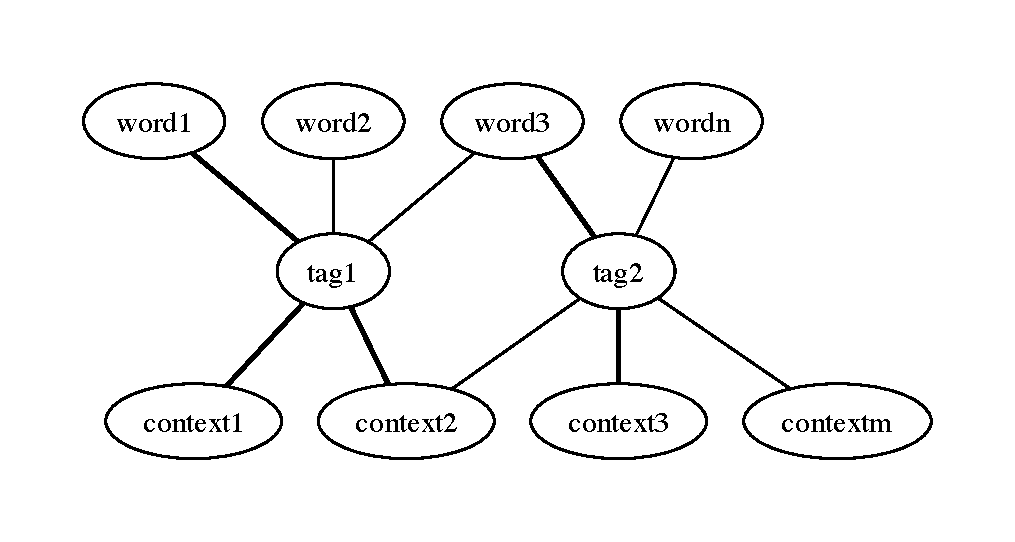
\includegraphics[width=0.7\columnwidth]{bipartite_lda.pdf}

\end{frame}

\begin{frame}[t]{Constituency and context}
\vspace{0.25in}
\begin{center}
\only<1>{
  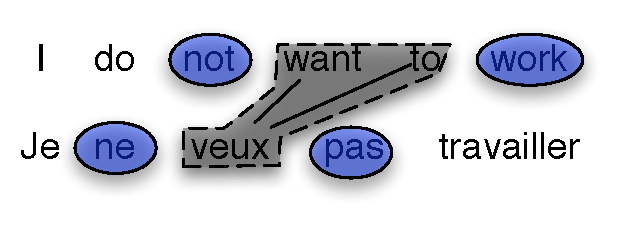
\includegraphics[scale=0.5]{WantTo_Veux_context.pdf}
  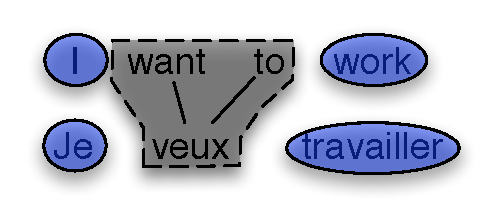
\includegraphics[scale=0.5]{WantTo_Veux_context2.pdf}
}
\only<2>{
  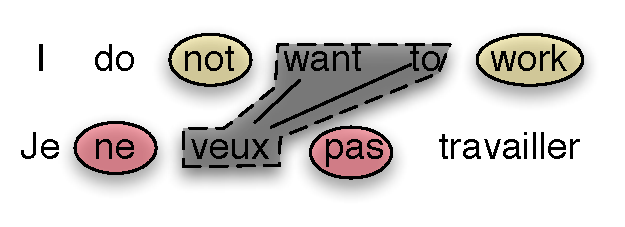
\includegraphics[scale=0.5]{WantTo_Veux_context_split.pdf}
  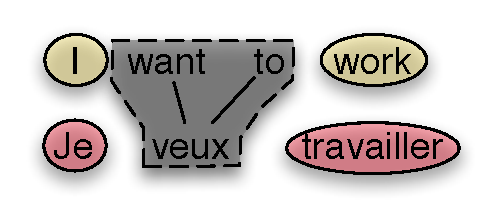
\includegraphics[scale=0.5]{WantTo_Veux_context2_split.pdf}
}
\only<3>{
  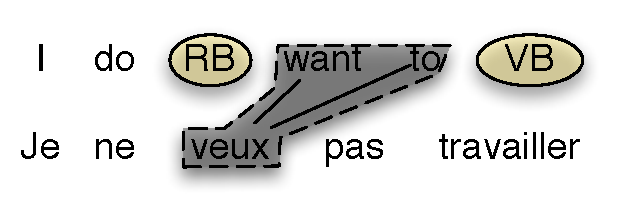
\includegraphics[scale=0.5]{WantTo_Veux_context_split_mono.pdf}
  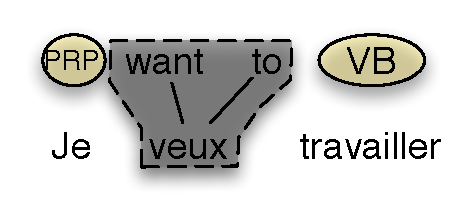
\includegraphics[scale=0.5]{WantTo_Veux_context2_split_mono.pdf}
}
\end{center}
\vspace{0.1in}
%\only<1>{
%  There has been significant research into monolingual grammar induction:
%  \vspace{0.1in}
%  \begin{unpacked_itemize}
%  \item Alexander Clark. Unsupervised induction of stochastic context-free grammars using distributional clustering, 2001
%  \item Dan Klein and Chris Manning. A Generative Constituent-Context Model for Improved Grammar Induction, 2002
%  \end{unpacked_itemize}
%  \alert{Constituent context is a prime indicator of constituency.}
%}
%\only<1>{
\begin{unpacked_itemize}
\item Design and apply large scale scale clustering and topic modelling algorithms (LDA, HDPs, HPYPs etc), 
\item identify sets of frequent contexts that distinguish synchronous constituent properties.
\item Motivated by successful models of monolingual grammar induction,
\item deep connections to unsupervised word sense disambiguation, thesaurus extraction etc.
\end{unpacked_itemize}
%}
\end{frame}

\begin{frame}[t]{Latent Dirichlet Allocation (LDA)}

LDA is a generative model which treats documents as bags of words
\begin{itemize}
    \item each word is assign a \alert{topic} (cluster tag)
    \item words are generated from a topic-specific multinomial
    \item topics are \alert{tied} across a document using a Dirichlet prior
    \item $\alpha < 1$ biases towards \alert{sparse} distributions, i.e., topic reuse
    \item inferred $\theta_d$ describes a document and $\phi_t$ describes a topic
\end{itemize}

\vspace{-3ex}
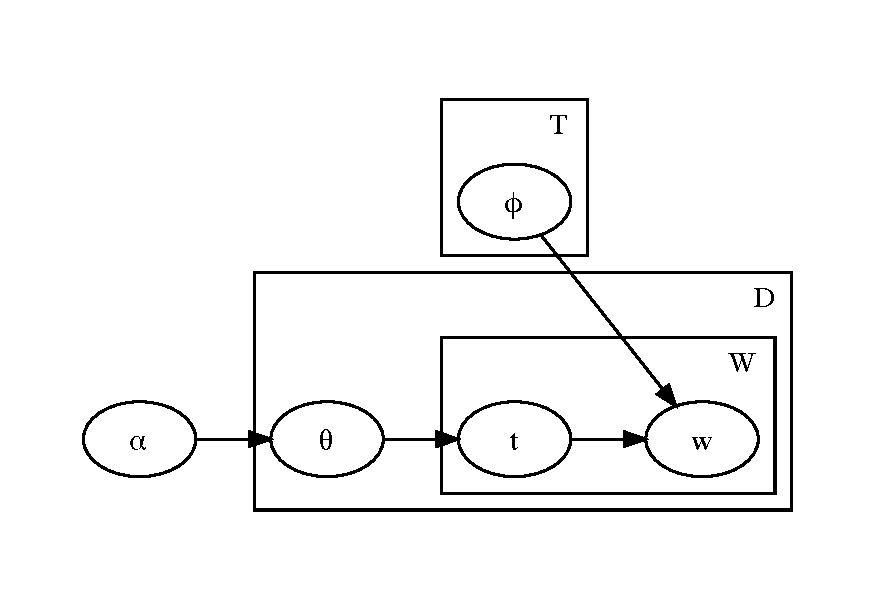
\includegraphics[scale=0.55]{lda.pdf}

\end{frame}

\begin{frame}[t]{LDA over Contexts}

Generative story:
\begin{itemize}
    \item for each word type $w$
    \item for each of the $L$ contexts
    \item first we draw a topic $t$, then generate the context $\vec{c}$ given the topic
    \item the Dirichlet prior ties the topics for each $w$
    \item we're primarily interested in the learnt $\theta$ values
\end{itemize}

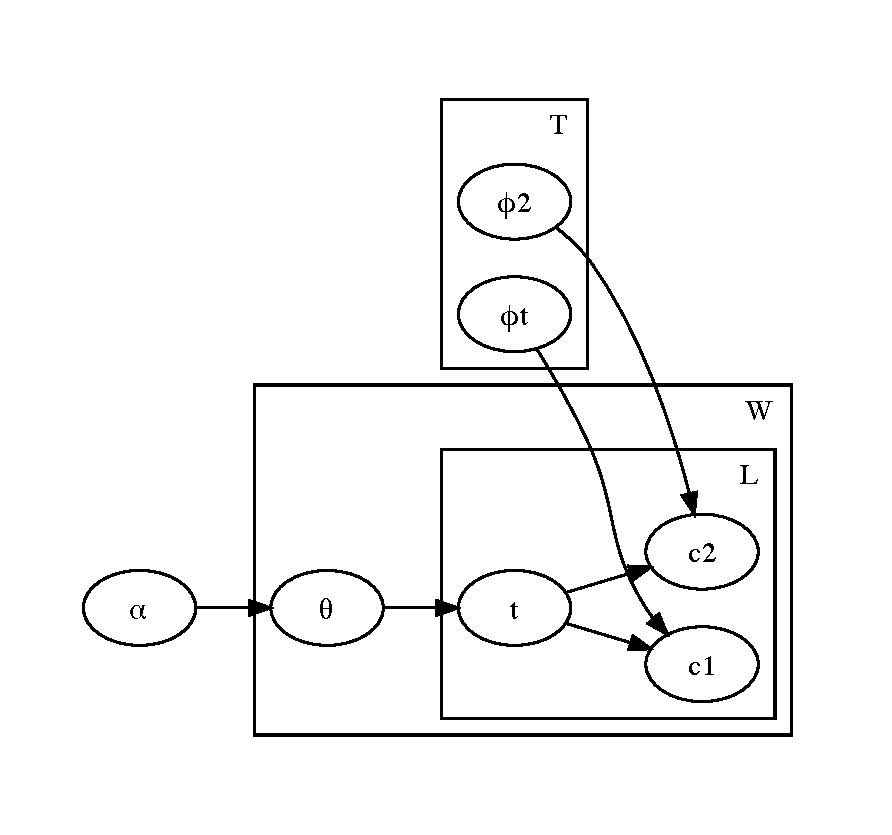
\includegraphics[scale=0.4]{context_lda.pdf}

\end{frame}

\begin{frame}[t]{Scalable grammar extraction with MapReduce}
\begin{itemize}
\item Divide and conquer approach to...counting
\begin{itemize}
\item map function $\mathcal{M}(x) \rightarrow \langle k_1, v_1 \rangle, \langle k_2, v_2 \rangle, \ldots$
\item write a reduce function $\mathcal{R}(k_i : v_7, v_{13} , \ldots) \rightarrow \langle k_i, \overline{v} \rangle$
\end{itemize}
\end{itemize}
\begin{center}
  \includegraphics[scale=0.4]{mroutline.pdf}
\end{center}
\end{frame}
\begin{frame}[t]{Scalable grammar extraction with MapReduce : mapper}
\begin{center}
  \includegraphics[scale=0.4]{mapper.pdf}
\end{center}
\end{frame}

\begin{frame}[t]{Scalable grammar extraction with MapReduce : reducer}
\begin{center}
  \includegraphics[scale=0.4]{reducer.pdf}
\end{center}
\end{frame}

\begin{frame}[t]{Scalable grammar extraction with MapReduce : Hadoop}
\begin{center}
  \includegraphics[scale=0.4]{hadoop-extract.pdf}
\end{center}
\end{frame}

\begin{frame}[t]{Scalable grammar extraction with MapReduce : Hadoop}
\begin{center}
  \includegraphics[scale=0.4]{hadoop-extract-arrows.pdf}
\end{center}
\end{frame}


%\begin{frame}[t]{Discriminative training}
%\begin{unpacked_itemize}
%\item MIRA
%\item Expected loss minimisation.
%\end{unpacked_itemize}
%\end{frame}


\begin{frame}[t]{Language pairs (small)}
\begin{itemize}
\item BTEC Chinese-English:
  \begin{itemize}
  \item 44k sentence pairs, short sentences
  \item Widely reported `prototyping' corpus
  \item Hiero baseline score: 52.4 (16 references)
  \item Prospects: BTEC always gives you good results
  \end{itemize}
\item NIST Urdu-English:
  \begin{itemize}
  \item 50k sentence pairs
  \item Hiero baseline score: MT05 - 23.7 (4 references)
  \item Major challenges: major long-range reordering, SOV word order
  \item Prospects: small data, previous gains with supervised syntax
  \end{itemize}
\end{itemize}
\end{frame}

\begin{frame}[t]{Language pairs (large)}
\begin{itemize}
\item NIST Chinese-English:
  \begin{itemize}
  \item 1.7M sentence pairs, Standard NIST test sets
  \item Hiero baseline score: MT05 - 33.9 (4 references)
  \item Major challenges: large data, mid-range reordering, lexical ambiguity
  \item Prospects: supervised syntax gains reported
  \end{itemize}
\item NIST Arabic-English:
  \begin{itemize}
  \item 900k sentence pairs
  \item Hiero baseline score: MT05 - 48.9 (4 references)
  \item Major challenges: strong baseline, local reordering, VSO word order
  \item Prospects: difficult
  \end{itemize}
\item Europarl Dutch-French:
  \begin{itemize}
  \item 1.5M sentence pairs, standard Europarl test sets
  \item Hiero baseline score: Europarl 2008 - 26.3 (1 reference)
  \item Major challenges: V2 / V-final word order, many non-literal translations
  \item Prospects: ???
  \end{itemize}
\end{itemize}
\end{frame}

%\begin{frame}[t]{Draft Schedule}
%\begin{itemize}
%\item Pre-workshop:
%  \begin{itemize}
%  \item Collect existing open-source tools for synchronous grammar induction,
%  \item Collect corpora across a range of translations conditions: small, large, low-density languages etc.
%  \item Implement phrase and context extraction algorithms.
%  \item Design the integration of various existing approaches into the decoders.
%  \end{itemize}
%\item Week 1:
%  \begin{itemize}
%  \item Optimise and reconfigure decoders to handle labelled synchronous grammars,
%  \item Perform a empirical study of synchronous constituency models.
%  \end{itemize}
%\end{itemize}
%\end{frame}

%\begin{frame}[t]{Draft Schedule}
%\begin{itemize}
%\item Week 2-3:
%  \begin{itemize}
%  \item Continue optimising decoder to handle labelled synchronous grammars,
%  \item Implement unsupervised label induction algorithms, initially inducing a single label per-phrase.
%  \item Extend to ''topic"-modelling style representation where a phrase may have multiple labellings.
%  \item Perform experimental comparison of existing synchronous grammar translation models.
%  \end{itemize}
%\item Week 3-6:
%  \begin{itemize}
%  \item Perform experimental comparison of unsupervised synchronous grammar translation models.
%  \item Extend the evaluation to small/big data sets, hi-density vs. low-density language pairs.
%  \item Create ``semi-supervised'' models combining knowledge from treebank parser into the unsupervised algorithms.
%  \item Wrap-up and write final report.
%  \end{itemize}
%\end{itemize}
%\end{frame}


\begin{frame}[t]{Pre-workshop experiments}
\vspace{0.25in}
We have implemented a baseline constituent modelling and distrbuted grammar extraction pipeline. Initial results on the small BTEC corpora:

\vspace{0.25in}
\begin{exampleblock}
\footnotesize
\centering
\begin{tabular}{lcccccc}
\toprule
Categories & \small 1-gram & \small 2-grams & \small 3-grams & \small 4-grams & \small BP  &  BLEU  \\
\midrule                                                                                            
1          & \small 84.7 & \small 62.0    & \small 47.2    & \small 36.4    & \small 0.969 &  \textcolor{blue}{53.10} \\
10         & \small 84.0 & \small 60.9    & \small 46.4    & \small 35.9    & \small 0.979 &  \textcolor{red}{52.88} \\
25         & \small 84.4 & \small 61.8    & \small 47.6    & \small 36.7    & \small 0.973 &  \textcolor{blue}{53.47} \\
50         & \small 84.8 & \small 61.2    & \small 46.6    & \small 36.2    & \small 0.971 &  \textcolor{red}{52.83} \\
100        & \small 83.5 & \small 60.1    & \small 45.7    & \small 35.3    & \small 0.972 &  \textcolor{red}{51.86} \\
\bottomrule
\end{tabular}
\end{exampleblock}
\end{frame}


%{\centering
%A unique opportunity to bring together researchers operating at the coal face of SMT development with leading theoreticians in the field of formal grammar induction.
%}
%\begin{unpacked_itemize}
%\item Understand the relationship between constituent labels and performance in SMT,
%\item Compare monolingual and bilingual induced grammars against parser output in terms of translation quality,
%\item Produce a large scale implementation of the label induction algorithms,
%\end{unpacked_itemize}
%\begin{unpacked_itemize}
%\item \alert{Learn language-pair dependent structure that produces translation performance gains across all language pairs,}
%\item \alert{Initiate a research program that redirects the SMT research community back to language neutral unsupervised systems.}
%\end{unpacked_itemize}


\begin{frame}[t]{Summary}
\begin{itemize}
\item Scientific Merit:
  \begin{itemize}
  \item A systematic comparison of existing syntactive approaches to SMT.
  \item An empirical study of how constituency is useful in SMT.
  \item An evaluation of existing theories of grammar induction in a practical application (end-to-end evaluation).
  \end{itemize}
\item Potential Impact:
  \begin{itemize}
  \item Better MT systems, for more languages, across a range of domains.
  \item More accessible high performance translation models for researchers. % all over the world.
  \end{itemize}
\item Feasibility:
  \begin{itemize}
  \item A great team with a wide range of both theoretical and practical experience.
  %\item Incremental plan without any deal breaking dependencies.
  \item Solid preparation.
  \end{itemize}
\item Novelty:
  \begin{itemize}
  \item First attempt at large scale unsupervised synchronous grammar induction.
%  \item First study seeking to compare and understand the impact of synchronous structure on translation performance. 
  \end{itemize}
\end{itemize}
\end{frame}


\end{document}
